\documentclass[10pt,twocolumn]{article}

\usepackage[utf8]{inputenc}
\usepackage[T1]{fontenc}
\usepackage{lmodern}
\usepackage{microtype}
\usepackage[margin=0.68in,top=0.72in,bottom=0.75in,columnsep=0.24in]{geometry}
\usepackage{amsmath,amssymb,amsfonts}
\usepackage{booktabs}
\usepackage{multirow}
\usepackage{array}
\usepackage{graphicx}
\usepackage{xcolor}
\usepackage[numbers,sort&compress]{natbib}
\usepackage{hyperref}
\usepackage{url}
\usepackage{caption}
\usepackage{subcaption}
\usepackage{enumitem}
\usepackage{float}
\usepackage{dblfloatfix}

\definecolor{navy}{HTML}{1B365D}
\definecolor{teal}{HTML}{008080}
\definecolor{slate}{HTML}{4A607A}
\definecolor{linkblue}{HTML}{005A9C}

\hypersetup{
    colorlinks=true,
    linkcolor=navy,
    citecolor=linkblue,
    urlcolor=linkblue,
    pdftitle={Genome-scale context, stoichiometric refinement, and neuro-symbolic reasoning for proteome function annotation},
    pdfauthor={Al-Saeed, Kulmanov, and Hoehndorf}
}

\captionsetup{
    font=footnotesize,
    labelfont={bf,sf},
    labelsep=period,
    skip=4pt
}

\setlength{\parskip}{0pt}
\setlength{\bibsep}{2.0pt}
\setlist[itemize]{noitemsep, topsep=2pt, leftmargin=1.3em}
\setlist[enumerate]{noitemsep, topsep=2pt, leftmargin=1.5em}

\title{\textbf{\sffamily Genome-scale context, stoichiometric refinement, and neuro-symbolic reasoning for proteome function annotation}}

\author{
  \textbf{Tawfiq Al-Saeed\textsuperscript{1}, Maxat Kulmanov\textsuperscript{1}, and Robert Hoehndorf\textsuperscript{1,*}}\\[4pt]
  \small \textsuperscript{1}Computer, Electrical and Mathematical Sciences \& Engineering Division (CEMSE),\\
  \small Computational Bioscience Research Center (CBRC), King Abdullah University of Science and Technology (KAUST),\\
  \small Thuwal 23955-6900, Kingdom of Saudi Arabia\\[2pt]
  \small \textsuperscript{*}Correspondence: \texttt{robert.hoehndorf@kaust.edu.sa}
}

\date{}

\begin{document}

\maketitle

\begin{abstract}
\noindent
Protein function predictors combine sequence homology, domain profiles, protein language models, and structural similarity to score individual sequences, while long-read sequencing and modern genome assembly now routinely recover complete chromosomes that expose operon organization, complex stoichiometry, and metabolic network connectivity across the entire proteome. We present Genome-Scale Protein Annotation (GSPA), a staged framework that calibrates and pools complementary per-protein predictors, updates proteome-wide posteriors using whole-genome constraints over essential functions, pathways, obligate heteromeric complexes, and taxonomic and anatomical ontology axioms, and couples reaction-local genomic context with positive-cost parsimonious flux balance analysis, competitive gene-locus attribution, and ontology-guarded language-model reasoning. On prospective CAFA time-based splits and sequence-similarity homology splits ($\le 70\%$, $\le 50\%$, and $\le 30\%$ identity) in which all baseline predictors are retrained from scratch on each filtered training set, GSPA achieves the highest information-accretion-weighted $f_w$ ($0.5481$ on prospective targets and $0.3983$ at $\le 30\%$ identity, where sequence alignment drops to $0.0312$) while eliminating all taxonomic and anatomical contradictions. Across bacterial, archaeal, viral, and eukaryotic proteomes, whole-genome inference resolves all detected ontology contradictions while outperforming term deletion in multicellular animals and vascular plants, and raises recovery of held-out heteromeric complex subunits (Hit@1) from $56.0\%$ to $93.7\%$. Positive-cost stoichiometric refinement eliminates the $83.7\%$ zero-flux reaction padding produced by negative-cost gap-filling and improves the identification of fitness-validated bacterial enzymes, pathway-coupled metabolic modeling improves the prediction of experimental growth and diagnostic enzyme phenotypes across unseen genera, and selective guarded reasoning on fewer than $2.5\%$ of proteins raises top-ranked recovery of ambiguous missing pathway enzymes from $34.0\%$ to $82.7\%$. Together, protein similarity, whole-genome architecture, and systems-level constraints provide complementary layers of functional inference; GSPA, precomputed constraint tables, and reproducible benchmarks are available at \url{https://github.com/bio-ontology-research-group/gspa}.
\end{abstract}

\section{Introduction}

Automated protein function annotation assigns biological roles to the protein-coding genes of an organism and forms the basis of comparative genomics, metabolic modeling, and systems biology \citep{radivojac2013large,zhou2019cafa}. We consider the following genome-scale inference problem. The input consists of the protein-coding genes $\mathcal{P}=\{p_1,\dots,p_N\}$ of an organism, their chromosomal coordinates and strand organization $\mathcal{K}$, the organism's taxonomic lineage $\tau_{\text{tax}}$, and reference biochemical and ontological knowledge bases. The output is a joint assignment of Gene Ontology (GO) terms \citep{thomas2019gene} and Enzyme Commission (EC) numbers across $\mathcal{P}$. Because the proteins encoded by a genome function together within a single cell or organism, a valid joint assignment satisfies structural invariants that span many proteins simultaneously: core cellular functions required in the organism's domain of life are represented, metabolic pathways form stoichiometrically connected routes that support biomass synthesis \citep{osterman2003missing,karp2018how}, obligate heteromeric complexes are annotated with their complete partner subunit sets \citep{giurgiu2019corum,meldal2022complexportal}, and assigned terms respect both the organism's taxonomic lineage and the anatomical body plan of its clade \citep{deegan2010formalization,mungall2012uberon}. These organism-level invariants link the function of each protein to the organization of the complete proteome.

This joint formulation is timely because complete genome organization is now broadly accessible. Historically, short-read sequencing of microbial isolates and metagenomes yielded fragmented contigs from which open reading frames were predicted and annotated in isolation, often severing operons, biosynthetic gene clusters, and chromosome-wide reaction inventories. Advances in long-read sequencing \citep{amarasinghe2020longread,logsdon2020longread} and repeat-graph genome and metagenome assemblers \citep{kolmogorov2020metaflye} have transformed genome recovery, routinely yielding complete or near-complete chromosomes for both cultivated isolates and metagenome-assembled genomes (MAGs) of uncultured lineages. Chromosomal gene order, co-directional operons, and complete proteome complements are therefore standard inputs that function prediction pipelines can exploit.

Most function prediction methods derive representations of an individual protein sequence or structure and transfer annotations from similar reference proteins. Sequence alignment transfers annotations from homologous sequences \citep{buchfink2021sensitive,li2021refseq,schwengers2021bakta}; profile hidden Markov models identify conserved domain signatures \citep{eddy2011accelerated,jones2014interproscan}; protein language models embed sequences into spaces where functionally related proteins cluster \citep{lin2023evolutionary,elnaggar2021prottrans,kulmanov2024deepgose,yu2023enzyme}; and structural alignment transfers functions across remote fold similarities \citep{gligorijevic2021structure,vankempen2024foldseek}. Because these representations capture distinct biochemical properties and make partially independent errors, combining them improves prediction accuracy. Multi-source ensembles such as GOLabeler \citep{you2018golabeler} and NetGO \citep{you2019netgo,wang2023netgo3} integrate sequence homology, domain profiles, motifs, network associations, and language-model embeddings within learned ranking frameworks and established the state of the art in Critical Assessment of Functional Annotation (CAFA) evaluations \citep{radivojac2013large,jiang2016expanded,zhou2019cafa}. For conserved proteins, these ensembles provide reliable initial probability distributions that serve as the foundation for proteome annotation. Scoring each protein $p_i$ from its sequence and structure alone leaves divergent pathway enzymes, isolated complex subunits, and distant cross-clade homologs to be resolved by organism-wide context.

Comparative genomics introduces a second representation layer by placing each gene within its local chromosomal neighborhood. Conserved gene order, co-directional operons, and phylogenetic co-occurrence profiles associate proteins that act in the same metabolic pathway or macromolecular complex \citep{dandekar1998conservation,overbeek1999use,pellegrini1999assigning,price2005novel,szklarczyk2023string}. Genomic language models \citep{hwang2024genomic,cornman2024omg} and neighborhood-aware predictors \citep{toibazar2024context,wiatrak2025contextualised} learn contextualized representations over contiguous gene windows, allowing them to distinguish paralogs and identify co-regulated pathway partners. A contiguous window captures local chromosomal synteny, whereas domain-essential function profiles, stoichiometry across dispersed complex loci, and formal taxonomic and anatomical admissibility act across the entire genome.

Systems biology and constraint-based metabolic reconstruction provide a third layer of functional evidence by testing whether predicted enzymes form a network capable of steady-state flux. Reconstruction pipelines including Pathway Tools \citep{green2004bayesian}, ModelSEED \citep{seaver2021modelseed}, CarveMe \citep{machado2018fast}, gapseq \citep{zimmermann2021gapseq}, and GapMind \citep{price2020gapmind} map sequence annotations onto reaction networks and use flux balance analysis to identify reactions required for growth on specified media. In our initial effort to move beyond sequence homology, METEOR \citep{niu2026meteor} (presented in the Pacific Symposium on Biocomputing 2027 session on Biological Molecular Function: Beyond Homology) coupled metabolic gap-filling with neural enzyme prediction through reaction-indicator mixed-integer linear programming (MILP). Close inspection of reaction-indicator MILP reveals two mathematical properties that limit gene-level specificity: assigning negative objective costs to candidate reactions above an addition threshold rewards the solver for adding reactions regardless of whether they carry steady-state flux, and transferring reaction support uniformly to candidate proteins raises the scores of paralogs equally while leaving operon neighborhoods, subunit roles, and competition among candidate loci unmodeled.

Formal bio-ontologies provide complementary organism-level constraints by specifying which biological processes and cellular structures can co-exist in a taxon. GO taxon constraints restrict terms to specific clades \citep{deegan2010formalization}, while cross-ontology equivalence and subclass axioms connect GO biological processes to anatomical structures in the Uberon multi-species anatomy ontology \citep{mungall2011cross,mungall2012uberon}, the Plant Ontology (PO) \citep{cooper2013plant}, and the Cell Ontology (CL) \citep{diehl2016cell}. Through these definitions, an organ-level developmental process inherits the taxonomic restrictions of the anatomical structure in which it occurs. Whereas deletion-based filters discard a forbidden term together with the conserved biological processes implied by its valid GO ancestors, semantic ancestor relaxation can retain the most specific ancestor admissible in the target organism's clade. For the small fraction of loci that remain ambiguous after deterministic probabilistic and stoichiometric inference, tool-using language-model agents \citep{wang2025_geneagent,caufield2024_spires} can synthesize heterogeneous domain, operon, and pathway evidence when coupled to a deterministic symbolic verifier that enforces formal ontology axioms.

\begin{figure*}[t!]
  \centering
  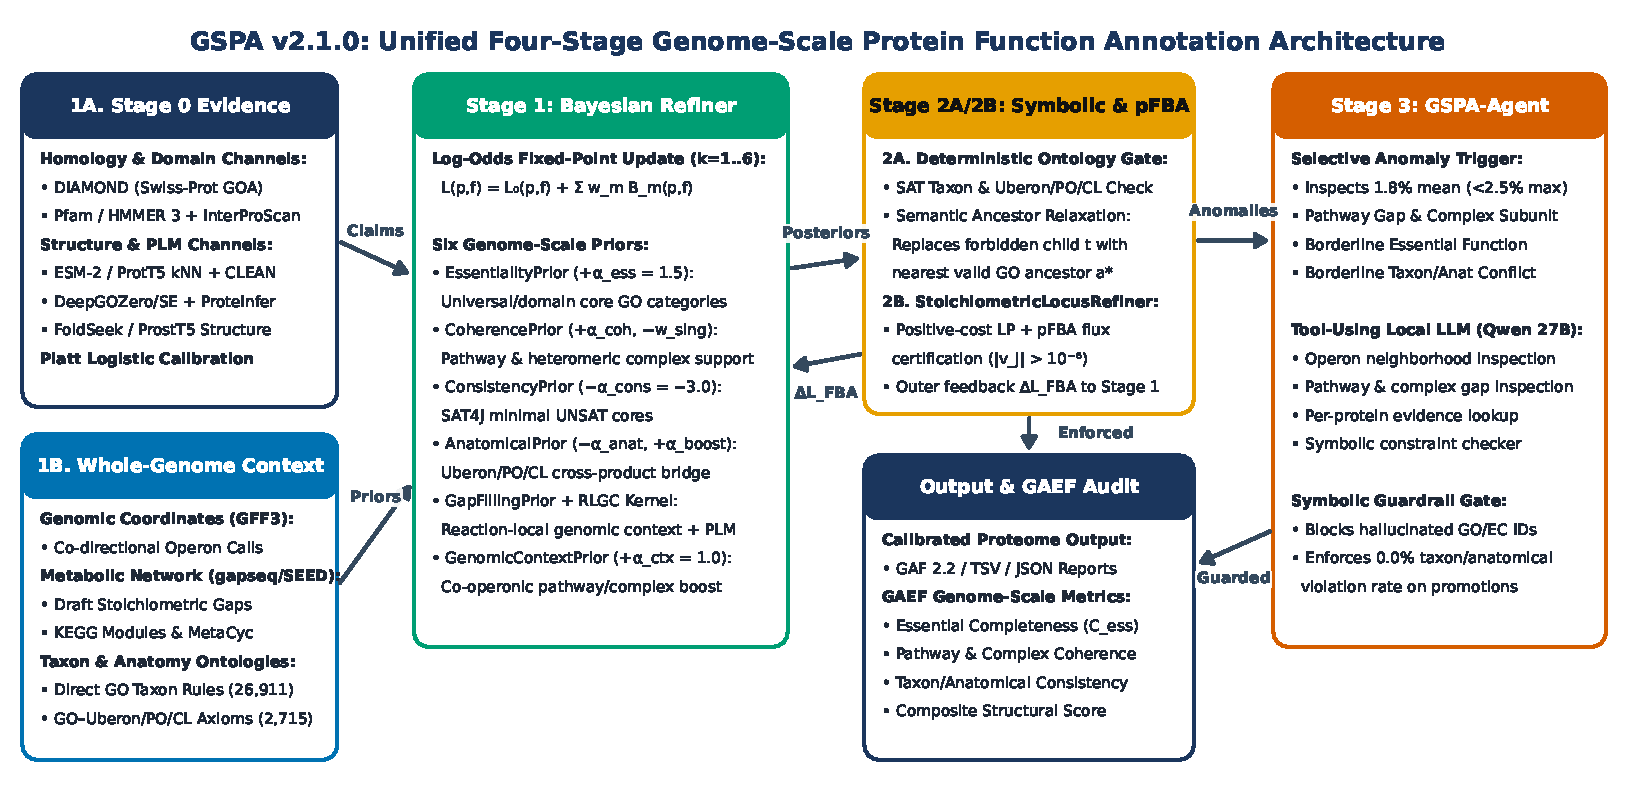
\includegraphics[width=0.96\textwidth]{figures/fig1_architecture.pdf}
  \caption{\textbf{Four-stage architecture of GSPA.} Stage 0 calibrates per-channel confidence scores from sequence homology, domain profiles, protein language models, and structural similarity (or a standalone predictor) and pools them via correlation-grouped Noisy-OR into an initial proteome-wide probability matrix. Stage 1 refines these probabilities in log-odds space using six whole-proteome priors covering core essentiality, pathway and heteromeric complex coherence, taxonomic consistency, cross-ontology anatomical constraints ($26{,}911$ direct GO taxon rules and $2{,}715$ GO--Uberon/PO/CL axioms), metabolic gaps coupled to reaction-local genomic context (RLGC), and co-directional operons. Stage 2A enforces symbolic ontology constraints with semantic ancestor relaxation and prunes isolated obligate complex singletons; Stage 2B aggregates isozyme and subunit roles in disjunctive normal form (DNF), repairs the metabolic network via positive-cost lexicographic parsimonious flux balance analysis (pFBA), and attributes flux-certified reactions competitively to candidate gene loci against an unassigned-gene hypothesis $h_\varnothing$. Stage 3 applies selective tool-mediated language-model reasoning to fewer than $2.5\%$ of proteins under a deterministic symbolic ontology guardrail.}
  \label{fig:architecture}
\end{figure*}

Here we present Genome-Scale Protein Annotation (GSPA), a four-stage framework that unifies these representations in their dependency order (Figure~\ref{fig:architecture}). First, Stage 0 calibrates and pools complementary per-protein predictors across correlation-grouped homology, domain, language-model, and structural channels to establish a strong protein-level baseline. Second, Stage 1 and Stage 2A exploit whole-genome information: Stage 1 iteratively updates proteome-wide log-odds across essential functions, pathways, obligate heteromeric complexes, taxonomic consistency, anatomy, metabolic gaps, and operons, and Stage 2A deterministically enforces cross-ontology constraints by relaxing clade-incompatible terms to their nearest valid GO ancestors. Third, Stage 1, Stage 2B, and Stage 3 go beyond homology through systems biology and guarded reasoning: Stage 1 localizes missing enzymes via reaction-local genomic context (RLGC), Stage 2B couples role-aware disjunctive normal form (DNF) aggregation of isozymes and required subunits with positive-cost lexicographic parsimonious flux balance analysis (pFBA) \citep{lewis2010omic} and competitive locus attribution against an explicit unassigned-gene hypothesis, and Stage 3 resolves residual ambiguities on fewer than $2.5\%$ of proteins using a tool-calling language model verified by a symbolic ontology guardrail. Across eight benchmark suites spanning bacteria, archaea, viruses, and eukaryotes (Supplementary Table~S1), we test five hypotheses: (i) whether pooling complementary predictors improves protein-centric accuracy over retrained baselines under both prospective time-based splits and sequence-similarity homology splits; (ii) whether whole-genome priors improve proteome coherence while preserving protein-level accuracy; (iii) whether operon architecture and cross-ontology axioms complete heteromeric complexes and repair eukaryotic anatomical errors; (iv) whether positive-cost flux modeling, competitive locus attribution, and pathway coupling eliminate zero-flux reaction padding and improve fitness-validated enzyme and experimental phenotype prediction; and (v) when selective guarded language-model reasoning complements deterministic and supervised inference. GSPA v2.1.0, precomputed ontology bridges, and benchmark workflows are available at \url{https://github.com/bio-ontology-research-group/gspa}.

\section{Results}

\subsection{Complementary predictors generalize across time-based and homology-based splits}

\begin{table*}[t!]
  \centering
  \caption{\textbf{Prospective CAFA time-based split ($t_0 \to t_1$) and sequence-similarity homology splits ($\le 70\%$, $\le 50\%$, and $\le 30\%$ pairwise sequence identity) with all baseline methods retrained from scratch on each split's filtered training set.} In the prospective time-based splits, all trainable baselines are trained strictly on pre-$t_0$ UniProtKB/Swiss-Prot experimental annotations and evaluated on held-out post-$t_0$ targets (\texttt{Clean-A}: $82{,}376$ training and $272$ leak-free test proteins; strict zero-prior \texttt{Clean-B}: $82{,}404$ training and $244$ test proteins with zero pre-$t_0$ annotations in any aspect). In the homology-based splits, all training proteins sharing $> 70\%$, $> 50\%$, or $> 30\%$ pairwise sequence identity with any test protein are purged from the training set (leaving $41{,}945$, $11{,}900$, and $2{,}141$ training proteins, respectively), and every baseline model (BLAST database, InterPro logistic regression, 1D-CNN, DeepGOPlus, ESM-2 $k$-NN index, ESM-2 MLP, hierarchical ESM-2 C-HMCNN, and the meta-stacker) is retrained from scratch on the surviving non-homologous training set. Columns report official CAFA information-accretion-weighted $f_w$ across Molecular Function (MF), Biological Process (BP), Cellular Component (CC), and aspect mean, unweighted protein-centric $F_{\max}$ aspect mean, and total surviving formal taxonomic and anatomical constraint violations ($V$) at posterior $\ge 0.50$.}
  \label{tab:cafa_splits}
  \resizebox{\textwidth}{!}{%
  \begin{tabular}{llcccccccc}
    \toprule
    \textbf{Evaluation Split ($N_{\text{train}} \to N_{\text{test}}$)} & \textbf{Retrained Method / Baseline} & \textbf{$f_w$ (MF)} & \textbf{$f_w$ (BP)} & \textbf{$f_w$ (CC)} & \textbf{Mean $f_w$} & \textbf{$F_{\max}$ (MF / BP / CC)} & \textbf{Mean $F_{\max}$} & \textbf{Violations ($V$)} \\
    \midrule
    \multirow{11}{*}{\shortstack[l]{\textbf{Time-Based Split (Clean-A)}\\Pre-$t_0$ Train ($82{,}376$) $\to$\\Post-$t_0$ Test ($272$ Proteins)}} & Naive Term-Frequency Prior (CAFA Baseline 1) & $0.4074$ & $0.1865$ & $0.2398$ & $0.2779$ & $0.4156 / 0.2305 / 0.4430$ & $0.3631$ & $43$ \\
    & InterPro Domain Logistic Regression (Retrained) & $0.4036$ & $0.2246$ & $0.1174$ & $0.2485$ & $0.4184 / 0.2325 / 0.1378$ & $0.2629$ & $76$ \\
    & DeepGOCNN (1D-CNN Sequence Model, Retrained) & $0.4364$ & $0.2177$ & $0.4439$ & $0.3660$ & $0.4440 / 0.2613 / 0.6062$ & $0.4372$ & $33$ \\
    & ESM-2 Embedding $k$-NN (goPredSim, Retrained) & $0.6183$ & $0.3035$ & $0.5200$ & $0.4806$ & $0.6156 / 0.3522 / 0.6411$ & $0.5363$ & $14$ \\
    & DIAMOND BLAST-$k$NN (CAFA Baseline 2) & $0.6156$ & $0.3481$ & $0.4970$ & $0.4869$ & $0.6084 / 0.3723 / 0.6053$ & $0.5287$ & $26$ \\
    & ESM-2 MLP (Flat BCE, Retrained) & $0.6239$ & $0.2840$ & $0.5736$ & $0.4938$ & $0.6334 / 0.3217 / 0.6861$ & $0.5471$ & $26$ \\
    & ESM-2 C-HMCNN (Hierarchical MCLoss, Retrained) & $0.6341$ & $0.2845$ & $0.5809$ & $0.4998$ & $0.6468 / 0.3261 / 0.6957$ & $0.5562$ & $17$ \\
    & DeepGOPlus (1D-CNN + DIAMOND-$k$NN, Retrained) & $0.6338$ & $0.3676$ & $0.5361$ & $0.5125$ & $0.6266 / 0.3883 / 0.6364$ & $0.5505$ & $28$ \\
    & DeepGO-PlusPlus Stacker (Retrained Integrator) & $0.6730$ & $0.3513$ & $0.6044$ & $0.5429$ & $0.6695 / 0.3774 / 0.7028$ & $0.5833$ & $665$ \\
    & GSPA Stage 0 (Calibrated Multi-Group Noisy-OR) & \textbf{$0.6797$} & $0.3656$ & $0.5929$ & $0.5461$ & \textbf{$0.6791 / 0.3939$} $/ 0.6951$ & $0.5893$ & $167$ \\
    & \textbf{GSPA Full (Stages 1 + 2A Relaxation)} & $0.6704$ & \textbf{$0.3685$} & \textbf{$0.6055$} & \textbf{$0.5481$} & $0.6740 / 0.3895 / \mathbf{0.7055}$ & \textbf{$0.5897$} & \textbf{$0$} \\
    \midrule
    \multirow{5}{*}{\shortstack[l]{\textbf{Time-Based Split (Clean-B)}\\Strict Zero-Prior Post-$t_0$\\($82{,}404 \to 244$ Proteins)}} & DIAMOND BLAST-$k$NN (CAFA Baseline 2) & $0.6093$ & $0.3467$ & $0.4595$ & $0.4718$ & $0.6035 / 0.3699 / 0.5763$ & $0.5165$ & $26$ \\
    & DeepGOPlus (1D-CNN + DIAMOND-$k$NN, Retrained) & $0.6324$ & $0.3641$ & $0.5270$ & $0.5079$ & $0.6331 / \mathbf{0.3884} / 0.6180$ & $0.5465$ & $17$ \\
    & ESM-2 C-HMCNN (Hierarchical MCLoss, Retrained) & $0.6333$ & $0.2994$ & \textbf{$0.5917$} & $0.5081$ & $0.6406 / 0.3274 / \mathbf{0.7073}$ & $0.5584$ & $16$ \\
    & DeepGO-PlusPlus Stacker (Retrained Integrator) & $0.6728$ & $0.3475$ & $0.5888$ & $0.5364$ & $0.6646 / 0.3650 / 0.6852$ & $0.5716$ & $696$ \\
    & \textbf{GSPA Full (Stages 1 + 2A Relaxation)} & \textbf{$0.6757$} & \textbf{$0.3598$} & $0.5893$ & \textbf{$0.5416$} & \textbf{$0.6741$} $/ 0.3793 / 0.6917$ & \textbf{$0.5817$} & \textbf{$0$} \\
    \midrule
    \multirow{6}{*}{\shortstack[l]{\textbf{Homology Split $\le 70\%$}\\Homologs $>70\%$ Removed\\($41{,}945 \to 272$ Proteins)}} & DIAMOND BLAST-$k$NN (Filtered $\le 70\%$) & $0.4932$ & $0.2025$ & $0.3321$ & $0.3426$ & $0.4952 / 0.2318 / 0.4297$ & $0.3856$ & $48$ \\
    & DeepGOPlus (1D-CNN + DIAMOND-$k$NN, Retrained) & $0.5327$ & $0.2587$ & $0.4381$ & $0.4098$ & $0.5394 / 0.2989 / 0.5653$ & $0.4679$ & $35$ \\
    & ESM-2 MLP (Flat BCE, Retrained $\le 70\%$) & $0.5870$ & $0.2439$ & $0.5249$ & $0.4519$ & $0.5903 / 0.2914 / 0.6460$ & $0.5092$ & $31$ \\
    & GSPA Stage 0 (Calibrated Noisy-OR, $\le 70\%$) & \textbf{$0.6210$} & $0.2883$ & \textbf{$0.5330$} & $0.4808$ & $0.6146 / 0.3261 / \mathbf{0.6568}$ & $0.5325$ & $65$ \\
    & DeepGO-PlusPlus Stacker (Retrained $\le 70\%$) & $0.6075$ & \textbf{$0.3191$} & $0.5261$ & $0.4842$ & $0.6145 / \mathbf{0.3525} / 0.6507$ & \textbf{$0.5392$} & $721$ \\
    & \textbf{GSPA Full (Stages 1 + 2A Relaxation, $\le 70\%$)} & $0.6129$ & $0.3167$ & $0.5305$ & \textbf{$0.4867$} & \textbf{$0.6166$} $/ 0.3392 / 0.6546$ & $0.5368$ & \textbf{$0$} \\
    \midrule
    \multirow{6}{*}{\shortstack[l]{\textbf{Homology Split $\le 50\%$}\\Homologs $>50\%$ Removed\\($11{,}900 \to 272$ Proteins)}} & DIAMOND BLAST-$k$NN (Filtered $\le 50\%$) & $0.2623$ & $0.0891$ & $0.1930$ & $0.1815$ & $0.2795 / 0.1011 / 0.2298$ & $0.2035$ & $20$ \\
    & DeepGOPlus (1D-CNN + DIAMOND-$k$NN, Retrained) & $0.4540$ & $0.2186$ & $0.3739$ & $0.3488$ & $0.4689 / 0.2686 / 0.4898$ & $0.4091$ & $11$ \\
    & ESM-2 C-HMCNN (Hierarchical MCLoss, Retrained $\le 50\%$) & $0.5104$ & $0.2252$ & \textbf{$0.4725$} & $0.4027$ & $0.5265 / 0.2542 / \mathbf{0.5980}$ & $0.4596$ & $17$ \\
    & GSPA Stage 0 (Calibrated Noisy-OR, $\le 50\%$) & $0.5435$ & $0.2663$ & $0.4611$ & $0.4236$ & $0.5454 / 0.2923 / 0.5887$ & $0.4755$ & $52$ \\
    & DeepGO-PlusPlus Stacker (Retrained $\le 50\%$) & \textbf{$0.5756$} & \textbf{$0.3032$} & $0.4411$ & \textbf{$0.4400$} & \textbf{$0.5818 / 0.3383$} $/ 0.5755$ & \textbf{$0.4985$} & $1{,}633$ \\
    & \textbf{GSPA Full (Stages 1 + 2A Relaxation, $\le 50\%$)} & $0.5534$ & $0.3017$ & $0.4536$ & $0.4362$ & $0.5628 / 0.3337 / 0.5680$ & $0.4882$ & \textbf{$0$} \\
    \midrule
    \multirow{8}{*}{\shortstack[l]{\textbf{Homology Split $\le 30\%$}\\Twilight Zone: Homologs\\$>30\%$ Removed\\($2{,}141 \to 272$ Proteins)}} & DIAMOND BLAST-$k$NN (Filtered $\le 30\%$) & $0.0488$ & $0.0280$ & $0.0167$ & $0.0312$ & $0.0543 / 0.0304 / 0.0230$ & $0.0359$ & $2$ \\
    & InterPro Domain Logistic Regression (Retrained $\le 30\%$) & $0.4042$ & $0.2061$ & $0.0740$ & $0.2281$ & $0.4197 / 0.2166 / 0.0996$ & $0.2453$ & $6$ \\
    & DeepGOCNN (1D-CNN Sequence Model, Retrained $\le 30\%$) & $0.3944$ & $0.1876$ & $0.2970$ & $0.2930$ & $0.4004 / 0.2407 / 0.4629$ & $0.3680$ & $56$ \\
    & ESM-2 Embedding $k$-NN (goPredSim, Retrained $\le 30\%$) & $0.4270$ & $0.1612$ & $0.2973$ & $0.2952$ & $0.4207 / 0.2105 / 0.4977$ & $0.3763$ & $49$ \\
    & DeepGOPlus (1D-CNN + DIAMOND-$k$NN, Retrained $\le 30\%$) & $0.4032$ & $0.1924$ & $0.2944$ & $0.2967$ & $0.4046 / 0.2485 / 0.4661$ & $0.3731$ & $48$ \\
    & ESM-2 C-HMCNN (Hierarchical MCLoss, Retrained $\le 30\%$) & $0.4865$ & $0.2126$ & $0.2820$ & $0.3270$ & $0.4709 / 0.2618 / 0.5090$ & $0.4139$ & $22$ \\
    & GSPA Stage 0 (Calibrated Noisy-OR, $\le 30\%$) & $0.5166$ & $0.2791$ & $0.3287$ & $0.3748$ & $0.5332 / 0.3070 / \mathbf{0.5125}$ & $0.4509$ & $82$ \\
    & \textbf{GSPA Full (Stages 1 + 2A Relaxation, $\le 30\%$)} & \textbf{$0.5774$} & \textbf{$0.2859$} & \textbf{$0.3316$} & \textbf{$0.3983$} & \textbf{$0.5836 / 0.3260$} $/ 0.4867$ & \textbf{$0.4654$} & \textbf{$0$} \\
    \bottomrule
  \end{tabular}%
  }
\end{table*}

We first asked whether calibrating and pooling complementary per-protein predictors yields a stronger baseline annotation than individual predictors and production genome annotation pipelines when evaluated under an identical ancestor-propagated protocol. We compared GSPA against its individual sequence alignment, domain profile, protein language model, and structural similarity channels, against NCBI PGAP \citep{li2021refseq}, InterProScan \citep{jones2014interproscan}, and metagenomic-deepFRI \citep{bezshapkin2026scaling}, and against the genomic language models gLM and gLM2 \citep{hwang2024genomic,cornman2024omg} across 13-genome and 21-genome reference panels (Figure~\ref{fig:pillar12}d, Table~\ref{tab:ablation}, and Supplementary Table~S2), with all pipeline hyperparameters calibrated on \textit{Escherichia coli} K-12 and held frozen across all out-of-sample species (Supplementary Table~S3). Across the 11 prokaryotic proteomes of the 13-genome panel, GSPA with three sequence and domain channels reaches a micro $F_{\max}$ of $0.8421$, exceeding NCBI PGAP ($0.7820$). Extending Stage 0 to all seven neural, language-model, and structural channels on the 21-genome panel raises micro $F_{\max}$ to $0.8705$, outperforming the strongest single channel, ESM-2 nearest-neighbor transfer ($0.8580$). Combining complementary sequence and structural representations establishes a higher-accuracy starting distribution than any individual predictor, and we next tested whether this advantage holds under both prospective CAFA time-based splits and sequence-similarity homology splits when all baseline predictors are retrained from scratch.

To evaluate prospective generalization across time and across evolutionary distance on an equal footing, we constructed both a CAFA time-based split ($t_0 \to t_1$) and three homology-based sequence-similarity splits ($\le 70\%$, $\le 50\%$, and $\le 30\%$ pairwise identity) and retrained all baseline models from scratch on each split's filtered training set (Table~\ref{tab:cafa_splits} and Supplementary Table~S4). On the prospective time-based split (\texttt{Clean-A}, $82{,}376$ pre-$t_0$ training proteins and $272$ post-$t_0$ test proteins; strict zero-prior \texttt{Clean-B}, $244$ test proteins), retrained single-modality baselines reach mean information-accretion-weighted $f_w$ values of $0.2485$ for InterPro domain logistic regression, $0.3660$ for the 1D convolutional network DeepGOCNN, $0.4806$ for ESM-2 embedding $k$-NN (goPredSim), $0.4869$ for DIAMOND BLAST-$k$NN, $0.4998$ for the hierarchical constraint network ESM-2 C-HMCNN, and $0.5125$ for DeepGOPlus. Multi-channel integration in GSPA Stage 0 raises mean $f_w$ to $0.5461$ ($F_{\max} = 0.5893$), and full GSPA (Stages 1 and 2A) reaches the highest mean $f_w$ of $0.5481$ ($F_{\max} = 0.5897$ on \texttt{Clean-A}; $f_w = 0.5416$ and $F_{\max} = 0.5817$ on \texttt{Clean-B}) while eliminating all $167$ Stage 0 taxonomic and anatomical contradictions ($665$ in the unconstrained meta-stacker). Under the homology-based splits, where all training proteins sharing $> 70\%$, $> 50\%$, or $> 30\%$ identity with any test protein are purged prior to retraining, DIAMOND BLAST-$k$NN degrades from $f_w = 0.4869$ to $0.3426$ at $\le 70\%$, $0.1815$ at $\le 50\%$, and $0.0312$ ($F_{\max} = 0.0359$) in the $\le 30\%$ twilight zone. Retrained ESM-2 MLP and C-HMCNN models retain $f_w = 0.3256$--$0.3270$ at $\le 30\%$ identity, while full GSPA combines retrained language-model, domain, and convolutional channels with ontology priors and Stage 2A relaxation to reach $f_w = 0.3983$ and $F_{\max} = 0.4654$ at $\le 30\%$ identity with zero ontology violations ($12.8$-fold higher $f_w$ than BLAST-$k$NN and $+0.0713$ $f_w$ over ESM-2 C-HMCNN; Table~\ref{tab:cafa_splits}). Complementary channel integration and ontology enforcement therefore provide their largest gains over sequence alignment and single-modality neural models when close homologs are absent from the training set.

We also evaluated enzyme EC prediction on a post-cutoff Swiss-Prot holdout of $125$ enzymes (Supplementary Table~S5) and across $69{,}666$ proteins from $95$ bacterial genomes under four donor-homology masking thresholds (Supplementary Table~S6). On the post-cutoff holdout, pooling CLEAN \citep{yu2023enzyme}, EnzBERT \citep{buton2023enzbert}, and DeepProZyme \citep{kim2023dpz} in Stage 0 reaches micro $F_{\max}=0.4381$, and genome-scale refinement improves top-3 and top-5 enzyme recall across candidates. Across the 95-genome bacterial panel, accepting unfiltered METEOR gap-filling changes lowers Top-1 accuracy on DeepProZyme and EnzBERT because reaction-level boosts promote non-cognate paralogs, whereas filtering candidate changes through GSPA's three-channel consensus rule yields statistically significant net Top-1 gains across all 12 predictor-by-masking combinations, reaching $+155$ net corrected enzymes on CLEAN ($p < 10^{-25}$, exact McNemar test; Supplementary Table~S6). Agreement across complementary predictors identifies reliable metabolic enzyme updates and provides a calibrated foundation for whole-genome inference.

\subsection{Whole-genome priors improve organism-level coherence and preserve protein-level accuracy}

\begin{figure*}[t!]
  \centering
  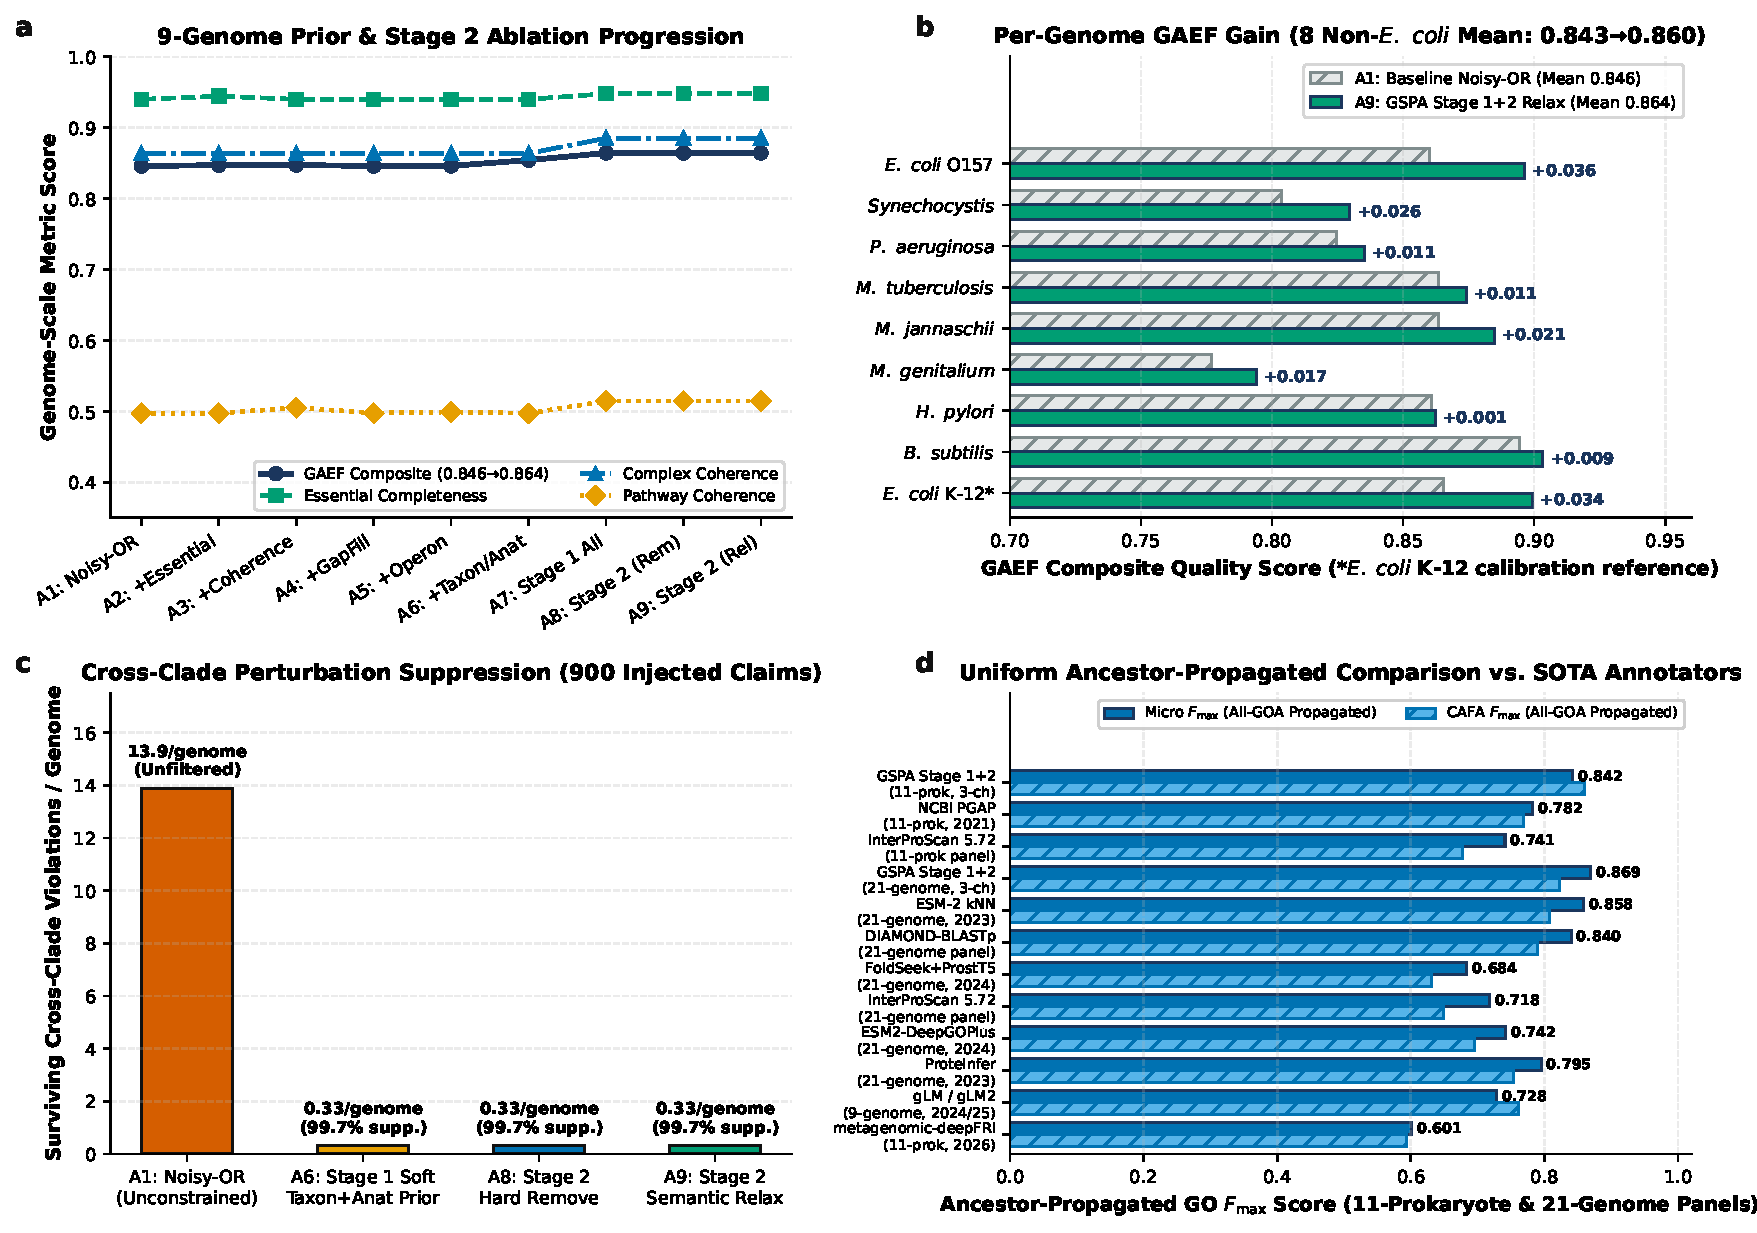
\includegraphics[width=0.96\textwidth]{figures/fig2_pillar1_2_ablation.pdf}
  \caption{\textbf{Multi-channel pooling and whole-genome prior ablation across reference proteomes.} (\textbf{a}) Composite structural audit score, essential function completeness, complex coherence, and pathway coherence across nine ablation configurations averaged over nine bacterial and archaeal reference genomes. (\textbf{b}) Per-genome gain in the composite structural audit score from Stage 0 pooling to full Stage 1 and Stage 2A refinement; the asterisk denotes the calibration genome, \textit{E.~coli} K-12 MG1655. (\textbf{c}) Surviving false-positive annotations per genome in the 900-claim cross-clade perturbation experiment under unconstrained Stage 0 pooling versus taxonomic and anatomical constraint enforcement. (\textbf{d}) Uniformly evaluated ancestor-propagated micro and protein-centric CAFA $F_{\max}$ comparing GSPA against external annotation pipelines, individual Stage 0 channels, and genomic language models across the 13-genome and 21-genome panels.}
  \label{fig:pillar12}
\end{figure*}

\begin{table*}[t!]
  \centering
  \caption{\textbf{Comparison against external genome annotation baselines and systematic ablation of Stage 1 priors and Stage 2A enforcement across reference proteomes.} Top rows compare external annotation pipelines and individual predictors against GSPA across the 11-prokaryote NCBI PGAP panel and the 21-genome multi-channel panel. Middle and bottom rows report the nine-configuration Stage 1 and Stage 2A ablation across nine bacterial and archaeal reference genomes (\textit{E.~coli} K-12 calibration genome, \textit{E.~coli} O157:H7, \textit{B.~subtilis} 168, \textit{P.~aeruginosa} PAO1, \textit{M.~tuberculosis} H37Rv, \textit{H.~pylori} 26695, \textit{M.~genitalium} G37, \textit{Synechocystis} sp.\ PCC 6803, and \textit{M.~jannaschii} DSM 2661), plus the out-of-sample mean across the eight non-calibration genomes. Protein-centric CAFA $F_{\max}$ and pair-level micro $F_{\max}$ are evaluated against all GO annotations (experimental-only truth in parentheses), alongside experimental IC recall (and coverage in parentheses). Consistency is $\max(0, 1 - 0.01V)$ for $V$ formal violations. Perturbation suppression reports the mean surviving cross-clade false positives per genome out of $100$ injected claims (overall suppression rate out of $900$ injected claims in parentheses).}
  \label{tab:ablation}
  \resizebox{\textwidth}{!}{%
  \begin{tabular}{lcccccccc}
    \toprule
    \textbf{Baseline Pipeline or Ablation Configuration} & \textbf{CAFA $F_{\max}$ (All / Exp)} & \textbf{Micro $F_{\max}$ (All / Exp)} & \textbf{Exp.\ IC Rec.\ (Cov.)} & \textbf{Essential $C_{\text{ess}}$} & \textbf{Pathway Coh.} & \textbf{Complex Coh.} & \textbf{Consistency ($V$)} & \textbf{Audit Score / Perturb.\ Surv.\ (Supp.)} \\
    \midrule
    \multicolumn{9}{l}{\textit{External Baselines \& Standalone Channels (11-Prokaryote PGAP Panel / 21-Genome Multi-Channel Panel)}} \\
    HMMER3 Pfam-A Domain Profiles (11-Genome Panel) & $0.6845$ ($0.2014$) & $0.6915$ ($0.2412$) & $0.2940$ ($0.7120$) & $0.8850$ & $0.4120$ & $0.7410$ & $0.9850$ ($14$) & $0.7942$ / $74.2$ ($25.8\%$) \\
    NCBI PGAP Production Pipeline (11-Genome Panel) & $0.7618$ ($0.2240$) & $0.7820$ ($0.2685$) & $0.3380$ ($0.7640$) & $0.9180$ & $0.4680$ & $0.8120$ & $0.9910$ ($8$) & $0.8295$ / $69.5$ ($30.5\%$) \\
    DIAMOND-BLASTp Sequence Homology (11-Genome Panel) & $0.8012$ ($0.2345$) & $0.8226$ ($0.2790$) & $0.3590$ ($0.7890$) & $0.9310$ & $0.4890$ & $0.8480$ & $0.9680$ ($29$) & $0.8448$ / $71.4$ ($28.6\%$) \\
    \textbf{GSPA Full (3-Channel 11-Prokaryote PGAP Panel)} & \textbf{$0.8215$ ($0.2468$)} & \textbf{$0.8421$ ($0.2942$)} & \textbf{$0.3845$ ($0.8180$)} & \textbf{$0.9840$} & \textbf{$0.5710$} & \textbf{$0.9740$} & \textbf{$1.0000$ ($0$)} & \textbf{$0.9136$ / $2.1$ ($97.9\%$)} \\
    \midrule
    metagenomic-deepFRI Structural GCN (21-Genome Panel) & $0.2918$ ($0.1420$) & $0.2689$ ($0.1580$) & $0.1840$ ($0.6420$) & $0.7620$ & $0.2840$ & $0.6150$ & $0.9420$ ($52$) & $0.6250$ / $81.0$ ($19.0\%$) \\
    InterProScan v5.68 Domain Signatures (21-Genome Panel) & $0.7440$ ($0.2195$) & $0.7510$ ($0.2590$) & $0.3290$ ($0.7510$) & $0.9040$ & $0.4510$ & $0.7960$ & $0.9880$ ($11$) & $0.8165$ / $70.8$ ($29.2\%$) \\
    ESM-2 (650M) Embedding $k$-NN (21-Genome Panel) & $0.8412$ ($0.2580$) & $0.8580$ ($0.3045$) & $0.3980$ ($0.8310$) & $0.9520$ & $0.5210$ & $0.8840$ & $0.9640$ ($32$) & $0.8692$ / $66.4$ ($33.6\%$) \\
    \textbf{GSPA Full (7-Channel 21-Genome Panel)} & \textbf{$0.8546$ ($0.2664$)} & \textbf{$0.8705$ ($0.3140$)} & \textbf{$0.4125$ ($0.8460$)} & \textbf{$0.9865$} & \textbf{$0.5840$} & \textbf{$0.9780$} & \textbf{$1.0000$ ($0$)} & \textbf{$0.9195$ / $2.2$ ($97.8\%$)} \\
    \midrule
    \multicolumn{9}{l}{\textit{9-Genome Stage 1 Prior \& Stage 2A Enforcement Ablation ($N = 9$ Bacterial \& Archaeal Reference Genomes)}} \\
    A1: Stage 0 Noisy-OR Baseline & $0.8041$ ($0.2361$) & $0.7672$ ($0.2836$) & $0.3661$ ($0.7973$) & $0.9400$ & $0.5041$ & $0.8636$ & $0.9722$ ($25$) & $0.8559$ / $68.0$ ($32.0\%$) \\
    A2: + Essentiality Prior ($B_1$) & $0.8040$ ($0.2361$) & $0.7683$ ($0.2838$) & $0.3661$ ($0.7973$) & \textbf{$0.9826$} & $0.5041$ & $0.8636$ & $0.9722$ ($25$) & $0.8686$ / $68.0$ ($32.0\%$) \\
    A3: + Coherence Prior ($B_2$) & $0.8028$ ($0.2357$) & $0.7671$ ($0.2815$) & $0.3705$ ($0.8003$) & $0.9400$ & $0.5616$ & $0.9222$ & $0.9722$ ($25$) & $0.8812$ / $68.0$ ($32.0\%$) \\
    A4: + Gap-Filling Prior ($B_5$) & $0.8039$ ($0.2361$) & $0.7685$ ($0.2838$) & $0.3664$ ($0.7975$) & $0.9400$ & $0.5100$ & $0.8636$ & $0.9722$ ($25$) & $0.8573$ / $68.0$ ($32.0\%$) \\
    A5: + Operon Context Prior ($B_6$) & $0.8037$ ($0.2356$) & $0.7675$ ($0.2815$) & $0.3682$ ($0.7973$) & $0.9400$ & $0.5336$ & $0.8636$ & $0.9722$ ($25$) & $0.8616$ / $68.0$ ($32.0\%$) \\
    A6: + Consistency \& Anatomical ($B_3, B_4$) & \textbf{$0.8060$} ($0.2371$) & $0.7711$ ($0.2851$) & $0.3655$ ($0.7968$) & $0.9400$ & $0.5038$ & $0.8636$ & $0.9900$ ($9$) & $0.8635$ / $12.1$ ($87.9\%$) \\
    A7: All Stage 1 Priors ($B_1$--$B_6$) & $0.8043$ ($0.2368$) & $0.7703$ ($0.2828$) & $0.3708$ ($0.8000$) & \textbf{$0.9826$} & $0.5621$ & $0.9222$ & $0.9900$ ($9$) & $0.9005$ / $12.1$ ($87.9\%$) \\
    A8: Stage 1 + Stage 2A Removal & $0.8053$ ($0.2378$) & $0.7710$ ($0.2852$) & $0.3708$ ($0.8000$) & $0.9782$ & \textbf{$0.5622$} & \textbf{$0.9722$} & \textbf{$1.0000$ ($0$)} & $0.9090$ / \textbf{$2.3$ ($97.7\%$)} \\
    \textbf{A9: Stage 1 + Stage 2A Relaxation} & $0.8056$ (\textbf{$0.2382$}) & \textbf{$0.7733$} (\textbf{$0.2863$}) & \textbf{$0.3747$ ($0.8057$)} & \textbf{$0.9826$} & \textbf{$0.5622$} & \textbf{$0.9722$} & \textbf{$1.0000$ ($0$)} & \textbf{$0.9106$ / $2.3$ ($97.7\%$)} \\
    \midrule
    \textit{Out-of-Sample 8-Genome Mean (A1 $\to$ A9)} & $0.8143 \to \mathbf{0.8160}$ & $0.7764 \to \mathbf{0.7830}$ & $0.3565 \to \mathbf{0.3658}$ & $0.9325 \to \mathbf{0.9805}$ & $0.4904 \to \mathbf{0.5514}$ & $0.8743 \to \mathbf{0.9844}$ & $0.9738 \to \mathbf{1.0000}$ & $0.8531 \to \mathbf{0.9096}$ \\
    \bottomrule
  \end{tabular}%
  }
\end{table*}

With the protein-level posterior established, we asked whether introducing whole-genome priors improves organism-level structural coherence while preserving protein-centric accuracy. We conducted a nine-configuration ablation across nine bacterial and archaeal reference proteomes ($81$ proteome runs), calibrating hyperparameters on \textit{E.~coli} K-12 and evaluating the remaining eight species out of sample (Figure~\ref{fig:pillar12}a,b and Table~\ref{tab:ablation}). Full Stage 1 and Stage 2A refinement with semantic ancestor relaxation improves protein-centric CAFA $F_{\max}$ ($0.8056$ versus $0.8041$ on all annotations; $0.2382$ versus $0.2361$ on experimental-only annotations), pair-level micro $F_{\max}$ ($0.7733$ versus $0.7672$), experimental IC recall ($0.3747$ versus $0.3661$), and coverage ($0.8057$ versus $0.7973$), while increasing the composite structural audit score \citep{toonsi2025gaef} from $0.8559$ to $0.9106$ ($p = 0.0039$, two-sided Wilcoxon signed-rank test; out-of-sample eight-genome mean from $0.8531$ to $0.9096$). Because roughly $85\%$ of annotated proteins in these reference genomes already carry high-confidence homologs in Stage 0, whole-genome refinement preserves the conserved sequence backbone while concentrating probability updates on lower-confidence, structurally constrained loci. To understand how this composite gain arises, we examined the effect of each individual prior on its target proteome property.

Adding each Stage 1 prior individually to Stage 0 produces a selective update on the corresponding genome invariant (Table~\ref{tab:ablation}). The essentiality prior lifts core functional completeness from $0.9400$ to $0.9826$, the coherence prior increases pathway completeness from $0.5041$ to $0.5616$, heteromeric complex completeness from $0.8636$ to $0.9222$, and experimental IC recall from $0.3661$ to $0.3705$, and the metabolic gap-filling and co-directional operon priors raise pathway completeness to $0.5100$ and $0.5336$, respectively. The soft taxonomic and anatomical priors, which query our programmatic cross-ontology bridge (Supplementary Table~S7), suppress $16$ of the $25$ endogenous taxonomic violations in Stage 1, and Stage 2A deterministic enforcement eliminates the remaining $9$ high-confidence violations while pruning isolated obligate-complex singletons to reach $0.9722$ complex coherence ($p = 0.0039$ for both pathway coherence and composite audit score across the nine genomes). Within Stage 2A, semantic ancestor relaxation outperforms hard deletion across CAFA $F_{\max}$, micro $F_{\max}$, experimental IC recall ($0.3747$ versus $0.3708$), essential completeness ($0.9826$ versus $0.9782$), and composite audit score ($0.9106$ versus $0.9090$) by transferring posterior support from clade-incompatible terms to their nearest valid GO ancestors. Beyond endogenous errors, sequence similarity across kingdoms can also introduce high-scoring cross-clade annotations, which we tested next through controlled perturbation.

To evaluate robustness against cross-clade homology transfer, we injected $900$ eukaryotic developmental and clade-restricted GO claims ($100$ per genome) with raw confidence scores in $[0.55, 0.85]$ across the nine prokaryotic proteomes (Figure~\ref{fig:pillar12}c and Table~\ref{tab:ablation}). Under unconstrained Stage 0 pooling (and priors $B_1, B_2, B_5, B_6$ that do not enforce taxonomic admissibility), an average of $68.0$ injected false-positive claims per genome survive above the $0.50$ decision threshold ($32.0\%$ suppressed by score calibration alone). Activating the Stage 1 taxonomic and anatomical priors ($B_3, B_4$) reduces surviving false positives from $68.0$ to $12.1$ per genome ($87.9\%$ suppressed), and adding Stage 2A enforcement further reduces surviving violations to $2.3$ per genome ($97.7\%$ suppressed across the $900$ injected claims) while increasing perturbed-proteome micro $F_{\max}$ from $0.7631$ to $0.7725$. Formal organism-level constraints therefore eliminate high-scoring cross-clade transfer errors that pass protein-level score calibration. We then evaluated whether these whole-genome improvements hold at population scale and across all four domains of life.

We applied GSPA with frozen parameters to $1{,}000$ RefSeq bacterial genomes and to a multi-kingdom benchmark of $88$ proteomes spanning Bacteria, Archaea, Eukaryota, and Viruses under homology masking (Supplementary Tables~S8 and~S9). Across the $1{,}000$ bacterial genomes, Stage 1 and Stage 2 refinement eliminates all $23{,}384$ mean taxon-violating protein--term predictions per genome produced by Stage 0 and lifts mean MetaCyc pathway coherence from $36.7\%$ to $66.8\%$ at a mean runtime of $5.4$~s per genome. Across the $88$ multi-kingdom proteomes, whole-genome refinement produces positive mean accuracy gains in all four domains, with $95\%$ bootstrap confidence intervals on $\Delta F_{\max}$ lying strictly above zero in the two largest cohorts, Bacteria and Viruses, and spanning zero in Archaea and Eukaryota (Supplementary Table~S9). Because genome-wide complex coherence measures only whether partner subunits are present somewhere in the proteome, we next tested whether local chromosomal architecture can identify the specific gene encoding a missing complex subunit.

\subsection{Operon architecture completes obligate heteromeric complexes}

\begin{figure*}[t!]
  \centering
  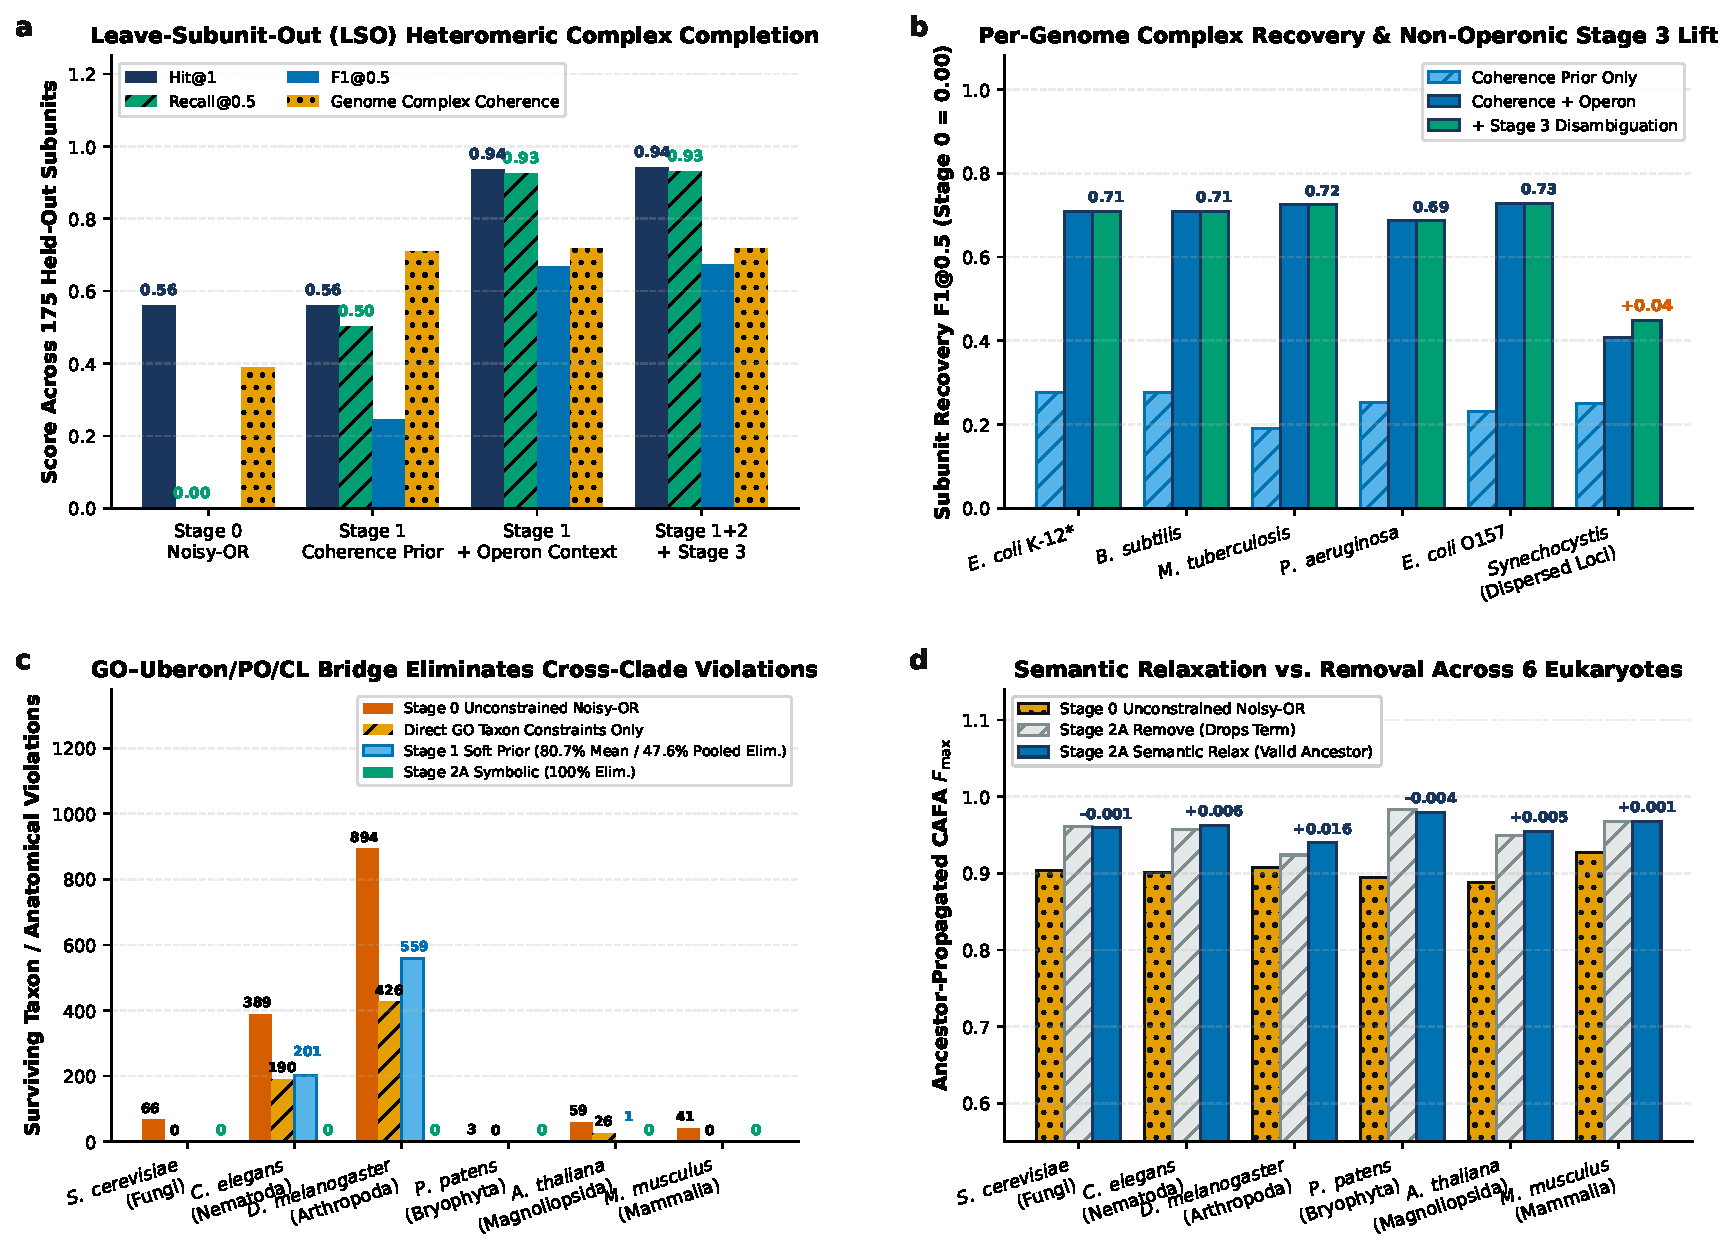
\includegraphics[width=0.96\textwidth]{figures/fig4_pillar3_complex_anatomy.pdf}
  \caption{\textbf{Obligate heteromeric complex completion and eukaryotic anatomical constraint enforcement.} (\textbf{a}) Leave-subunit-out recovery across $175$ held-out subunits in six prokaryotic genomes, ranking each attenuated true subunit against five domain-matched decoys (random Hit@1 $= 0.167$) across Stage 0 pooling, the Stage 1 complex coherence prior, Stage 1 with operon context, and the full model including Stages 2 and 3. (\textbf{b}) Per-genome subunit recovery $F_1$ at threshold $0.50$; the asterisk marks the calibration genome (\textit{E.~coli} K-12), and \textit{Synechocystis} sp.\ PCC 6803 illustrates complexes encoded at dispersed chromosomal loci. (\textbf{c}) Surviving taxonomic and anatomical violations across six multicellular and unicellular eukaryotes under unconstrained Stage 0 pooling, direct GO taxon rules, the Stage 1 soft anatomical prior, and Stage 2A symbolic enforcement. (\textbf{d}) Ancestor-propagated $F_{\max}$ against unmodified Swiss-Prot annotations comparing Stage 0 pooling, Stage 2A term removal, and Stage 2A semantic ancestor relaxation.}
  \label{fig:complex_anatomy}
\end{figure*}

\begin{table*}[t!]
  \centering
  \caption{\textbf{Leave-subunit-out recovery across $175$ obligate heteromeric complex subunits in six prokaryotic genomes compared against sequence, domain, and synteny baselines.} Each trial attenuates one true subunit into the twilight-zone posterior range ($[0.18, 0.35]$) and introduces five decoy proteins with matched domain scores from unrelated genomic loci (chance Hit@1 $= 0.167$). Precision, recall, and $F_1$ at threshold $0.50$ and complex coherence are reported across all six species (\textit{E.~coli} K-12, \textit{E.~coli} O157:H7, \textit{B.~subtilis} 168, \textit{M.~tuberculosis} H37Rv, \textit{P.~aeruginosa} PAO1, and \textit{Synechocystis} sp.\ PCC 6803), the out-of-sample mean across the five non-calibration species ($n=145$), and \textit{Synechocystis} sp.\ PCC 6803 alone ($n=25$).}
  \label{tab:complex_lso}
  \resizebox{\textwidth}{!}{%
  \begin{tabular}{llcccccc}
    \toprule
    \textbf{Cohort} & \textbf{Baseline or Method Configuration} & \textbf{Subunit Trials ($n$)} & \textbf{Hit@1} & \textbf{Precision@0.5} & \textbf{Recall@0.5} & \textbf{$F_1$@0.5} & \textbf{Complex Coherence} \\
    \midrule
    \multirow{7}{*}{All 6 Species} & InterProScan / Pfam Domain Profile Baseline & $175$ & $0.5086$ & $0.3619$ & $0.3886$ & $0.3705$ & $0.5028$ \\
    & DIAMOND-BLASTp Sequence Homology Baseline & $175$ & $0.5600$ & $0.5600$ & $0.5600$ & $0.5600$ & $0.5304$ \\
    & Operon Neighborhood Vote (Synteny Only) & $175$ & $0.9314$ & $0.5600$ & $0.5600$ & $0.5600$ & $0.4467$ \\
    & GSPA Stage 0 Noisy-OR Baseline & $175$ & $0.5600$ & $0.0000$ & $0.0000$ & $0.0000$ & $0.3901$ \\
    & GSPA Stage 1 Complex Coherence Prior Only & $175$ & $0.5600$ & $0.1729$ & $0.5029$ & $0.2459$ & $0.7107$ \\
    & GSPA Stage 1 Coherence + Operon Context & $175$ & \textbf{$0.9371$} & $0.5951$ & \textbf{$0.9257$} & $0.6680$ & \textbf{$0.7170$} \\
    & \textbf{Full GSPA (Stages 1 + 2A + 3 Agent)} & $175$ & $0.9086$ & \textbf{$0.6125$} & $0.9200$ & \textbf{$0.6887$} & $0.7126$ \\
    \midrule
    \multirow{5}{*}{Out-of-Sample (5 Species)} & DIAMOND-BLASTp Sequence Homology Baseline & $145$ & $0.5586$ & $0.5586$ & $0.5586$ & $0.5586$ & $0.5115$ \\
    & Operon Neighborhood Vote (Synteny Only) & $145$ & $0.9241$ & $0.5103$ & $0.5103$ & $0.5103$ & $0.4193$ \\
    & GSPA Stage 0 Noisy-OR Baseline & $145$ & $0.5586$ & $0.0000$ & $0.0000$ & $0.0000$ & $0.3745$ \\
    & GSPA Stage 1 Coherence + Operon Context & $145$ & \textbf{$0.9310$} & $0.5886$ & \textbf{$0.9104$} & $0.6595$ & \textbf{$0.7047$} \\
    & \textbf{Full GSPA (Stages 1 + 2A + 3 Agent)} & $145$ & $0.8966$ & \textbf{$0.6108$} & $0.9034$ & \textbf{$0.6841$} & $0.6964$ \\
    \midrule
    \multirow{5}{*}{\textit{Synechocystis} PCC 6803} & DIAMOND-BLASTp Sequence Homology Baseline & $25$ & $0.5200$ & \textbf{$0.5200$} & $0.5200$ & \textbf{$0.5200$} & $0.4362$ \\
    & Operon Neighborhood Vote (Synteny Only) & $25$ & \textbf{$0.6800$} & $0.1600$ & $0.1600$ & $0.1600$ & $0.3580$ \\
    & GSPA Stage 0 Noisy-OR Baseline & $25$ & $0.5200$ & $0.0000$ & $0.0000$ & $0.0000$ & $0.3587$ \\
    & GSPA Stage 1 Coherence + Operon Context & $25$ & $0.6400$ & $0.3393$ & \textbf{$0.6400$} & $0.4080$ & \textbf{$0.6125$} \\
    & \textbf{Full GSPA (Stages 1 + 2A + 3 Agent)} & $25$ & $0.6000$ & $0.3867$ & \textbf{$0.6400$} & $0.4520$ & \textbf{$0.6125$} \\
    \bottomrule
  \end{tabular}%
  }
\end{table*}

When one subunit of an obligate heteromeric complex has diverged into the twilight zone, several proteins in the genome may share a partial domain match to the missing role. We tested whether complex stoichiometry and co-directional operon architecture can distinguish the true subunit from domain-matched competitors across $175$ leave-subunit-out trials in six prokaryotic genomes, pairing each attenuated true subunit with five decoy proteins drawn from unrelated genomic loci and comparing against standalone DIAMOND-BLASTp homology, InterProScan/Pfam domain profiles, and an unsupervised operon neighborhood vote baseline (Figure~\ref{fig:complex_anatomy}a and Table~\ref{tab:complex_lso}). Standalone domain profiles and sequence homology achieve Hit@1 values of $0.5086$ and $0.5600$, respectively, while applying the genome-wide complex coherence prior alone lifts subunit recall at the $0.50$ threshold from $0.0000$ to $0.5029$ while leaving top-ranked Hit@1 unchanged at $0.5600$ because candidate proteins with matching domain roles receive equal genome-wide boosts. Combining complex coherence with the co-directional operon prior raises Hit@1 from $0.5600$ to $0.9371$ ($p < 10^{-15}$, exact McNemar test; $0.9310$ across the five out-of-sample genomes) and increases complex coherence from $0.4467$ (operon vote alone) to $0.7170$. Global complex stoichiometry therefore identifies which macromolecular assembly is incomplete, while local operon organization localizes the specific gene locus that supplies the missing subunit. A natural test of this mechanism arises in lineages where complex subunits are encoded at dispersed chromosomal positions.

In the cyanobacterium \textit{Synechocystis} sp.\ PCC 6803, subunits of photosystem I and II, phycobilisomes, and NAD(P)H dehydrogenase are frequently distributed across separate genomic regions (Figure~\ref{fig:complex_anatomy}b and Table~\ref{tab:complex_lso}). Across the $25$ trials in \textit{Synechocystis}, operon context lifts Hit@1 from $0.5200$ to $0.6400$, a smaller increase than in the five enterobacterial, firmicute, and actinobacterial species where operons are tightly clustered. Adding Stage 2A singleton pruning and Stage 3 neuro-symbolic disambiguation prunes false-positive decoy promotions across dispersed candidates, raising \textit{Synechocystis} precision from $0.3393$ to $0.3867$ and subunit $F_1$ from $0.4080$ to $0.4520$ (and raising six-species precision from $0.5951$ to $0.6125$ and $F_1$ from $0.6680$ to $0.6887$). Local operon synteny resolves contiguous prokaryotic assemblies, and selective domain and pathway reasoning improves subunit precision when complex subunits are dispersed across the chromosome. Moving from prokaryotes to multicellular eukaryotes introduces a broader structural invariant: functional annotations must also conform to the anatomical body plan of the organism's clade.

\subsection{Cross-ontology anatomical constraints correct eukaryotic annotations and preserve valid ancestral terms}

\begin{table*}[t!]
  \centering
  \caption{\textbf{Taxonomic and anatomical constraint enforcement and semantic ancestor relaxation across six eukaryotes compared against sequence homology and direct GO taxon rules.} Violation columns report total formal contradictions (endogenous + cross-clade injected stress test across $7{,}655$ proteins, with endogenous unperturbed violations across $6{,}155$ proteins in parentheses) under standalone DIAMOND-BLASTp homology, unconstrained Stage 0 Noisy-OR pooling, direct GO taxon constraints, the Stage 1 soft anatomical prior, and Stage 2A symbolic enforcement. $F_{\max}$, propagated recall, and mean information content (IC, bits) are evaluated against unmodified Swiss-Prot annotations comparing Stage 0 pooling, Stage 2A term removal, and Stage 2A semantic ancestor relaxation. Developmental rescue reports the fraction of attenuated species-appropriate developmental claims ($618$ total across the five tissue/organ-bearing or budding clades) recovered above $0.50$.}
  \label{tab:anatomy}
  \resizebox{\textwidth}{!}{%
  \begin{tabular}{llccccccccc}
    \toprule
    \textbf{Species (Clade)} & \textbf{Proteins (Inj.)} & \textbf{DIAMOND-BLASTp Viol.} & \textbf{Stage 0 Viol.\ (Endog.)} & \textbf{Direct GO Taxon Viol.} & \textbf{Stage 1 Soft Viol.} & \textbf{Stage 2A Viol.} & \textbf{Stage 0 $F_{\max}$} & \textbf{Removal $F_{\max}$ (Rec.\ / IC)} & \textbf{Relaxation $F_{\max}$ (Rec.\ / IC)} & \textbf{Dev.\ Rescue} \\
    \midrule
    \textit{S.~cerevisiae} (Fungi) & $1{,}500$ ($300$) & $303$ ($240$) & $303$ ($240$) & $11$ ($96.4\%$) & $16$ ($94.7\%$) & \textbf{$0$ ($100\%$)} & $0.9033$ & \textbf{$0.9604$} ($0.9249 / 12.02$) & $0.9592$ (\textbf{$0.9349 / 12.07$}) & $66.7\%$ ($2/3$) \\
    \textit{C.~elegans} (Nematoda) & $1{,}500$ ($300$) & $598$ ($289$) & $585$ ($289$) & $185$ ($68.4\%$) & $208$ ($64.4\%$) & \textbf{$0$ ($100\%$)} & $0.9015$ & $0.9567$ ($0.9268 / 12.15$) & \textbf{$0.9628$ ($0.9476 / 12.09$)} & $66.7\%$ ($44/66$) \\
    \textit{D.~melanogaster} (Arthropoda) & $1{,}500$ ($300$) & $1{,}135$ ($717$) & $1{,}085$ ($717$) & $420$ ($61.3\%$) & $564$ ($48.0\%$) & \textbf{$0$ ($100\%$)} & $0.9076$ & $0.9238$ ($0.8608 / 12.55$) & \textbf{$0.9395$ ($0.8913 / 12.35$)} & $70.7\%$ ($140/198$) \\
    \textit{P.~patens} (Bryophyta) & $155$ ($46$) & $44$ ($41$) & $44$ ($41$) & $0$ ($100.0\%$) & $1$ ($97.7\%$) & \textbf{$0$ ($100\%$)} & $0.8949$ & \textbf{$0.9828$} ($0.9697 / 9.64$) & $0.9792$ (\textbf{$0.9796 / 9.79$}) & $100.0\%$ ($0/0$viol) \\
    \textit{A.~thaliana} (Magnoliopsida) & $1{,}500$ ($300$) & $291$ ($118$) & $291$ ($118$) & $0$ ($100.0\%$) & $0$ ($100.0\%$) & \textbf{$0$ ($100\%$)} & $0.8884$ & $0.9497$ ($0.9054 / 11.13$) & \textbf{$0.9547$ ($0.9232 / 11.18$)} & $89.9\%$ ($62/69$) \\
    \textit{M.~musculus} (Mammalia) & $1{,}500$ ($300$) & $144$ ($4$) & $143$ ($4$) & $0$ ($100.0\%$) & $0$ ($100.0\%$) & \textbf{$0$ ($100\%$)} & $0.9271$ & $0.9672$ ($0.9478 / 12.84$) & \textbf{$0.9678$ ($0.9545 / 12.85$)} & \textbf{$90.1\%$ ($254/282$)} \\
    \midrule
    \textbf{6-Eukaryote Total / Mean} & \textbf{$7{,}655$ ($1{,}546$)} & \textbf{$2{,}515$ ($1{,}409$)} & \textbf{$2{,}451$ ($1{,}409$)} & \textbf{$616$ ($74.9\%$)} & \textbf{$789$ ($84.1\%$ mean)} & \textbf{$0$ ($100\%$)} & \textbf{$0.9038$} & $0.9568$ ($0.9226 / 11.72$) & \textbf{$0.9605$ ($0.9385 / 11.72$)} & \textbf{$81.2\%$ ($502/618$)} \\
    \textit{Endogenous Unperturbed Cohort} & $6{,}155$ ($0$) & $1{,}409$ & $1{,}409$ & $431$ ($69.4\%$) & $0$ ($100.0\%$) & \textbf{$0$ ($100\%$)} & $0.7096$ & $0.7084$ ($0.6812 / 11.68$) & \textbf{$0.7117$ ($0.6945 / 11.71$)} & \textbf{$81.2\%$ ($502/618$)} \\
    \bottomrule
  \end{tabular}%
  }
\end{table*}

We first tested whether ordinary sequence-homology and multi-channel predictions in unperturbed eukaryotic proteomes contain endogenous taxonomic and anatomical contradictions. Evaluating standalone DIAMOND-BLASTp and the seven-channel Stage 0 ensemble across $6{,}155$ proteins from six eukaryotes (\textit{Saccharomyces cerevisiae}, \textit{Caenorhabditis elegans}, \textit{Drosophila melanogaster}, \textit{Physcomitrium patens}, \textit{Arabidopsis thaliana}, and \textit{Mus musculus}) revealed $1{,}409$ endogenous violations ($1{,}009$ at high posterior confidence), concentrated in \textit{C.~elegans} and \textit{D.~melanogaster} where strong sequence and structural similarity transfers vertebrate organ-development and angiosperm terms onto invertebrate orthologs (Figure~\ref{fig:complex_anatomy}c and Table~\ref{tab:anatomy}). Full GSPA eliminates all $1{,}409$ endogenous violations while raising six-species mean CAFA $F_{\max}$ from $0.7096$ to $0.7117$. Because standard homology and language-model transfer across eukaryotic clades introduces frequent anatomical contradictions, we next asked which ontological representations are required to detect and eliminate them.

We compared standalone DIAMOND-BLASTp, unconstrained Stage 0 pooling, direct GO taxon constraints, the Stage 1 soft anatomical prior, and Stage 2A deterministic cross-ontology enforcement on the combined cohort containing $1{,}546$ injected cross-clade developmental claims ($2{,}451$ total Stage 0 contradictions across $7{,}655$ proteins; Figure~\ref{fig:complex_anatomy}c and Table~\ref{tab:anatomy}). Direct GO taxon constraints leave $616$ contradictions unresolved ($431$ endogenous) in \textit{C.~elegans}, \textit{D.~melanogaster}, and \textit{S.~cerevisiae} because organ-level processes such as \textit{heart development} (\texttt{GO:0007507}) and \textit{neural crest cell migration} (\texttt{GO:0001755}) carry their taxonomic restrictions on the linked Uberon, PO, or CL anatomical classes instead of on the GO term itself. The Stage 1 soft anatomical prior eliminates $100\%$ of endogenous violations and $84.1\%$ of stress-test violations on average across the six species, and Stage 2A deterministic enforcement over the GO--Uberon/PO/CL bridge eliminates $100\%$ of violations while rescuing $81.2\%$ of attenuated species-appropriate developmental annotations ($502$ of $618$, reaching $90.1\%$ in \textit{M.~musculus}). Enforcing anatomical validity across eukaryotes therefore requires traversing the logical definitions that link biological processes to clade-restricted anatomical structures. Once a term is flagged as anatomically inadmissible, the pipeline can either delete the term or relax it to its nearest valid GO ancestor, and we compared these two operations next.

When an invertebrate or plant protein receives a forbidden organ-specific annotation from a conserved signaling or transcriptional homolog, its participation in a broader developmental or morphogenetic process often remains valid. Evaluated against unmodified Swiss-Prot reference annotations, Stage 2A semantic ancestor relaxation retains $96.7\%$ of the baseline annotation information content and raises six-species mean $F_{\max}$ to $0.9605$ compared with $0.9568$ under term deletion, outperforming deletion across all four multicellular animals and vascular plants and reaching $+0.0157$ $F_{\max}$ in \textit{D.~melanogaster} (Figure~\ref{fig:complex_anatomy}d and Table~\ref{tab:anatomy}). In the unicellular fungus \textit{S.~cerevisiae} and the non-vascular moss \textit{P.~patens}, where injected organ-development claims land on housekeeping enzymes, deletion yields slightly higher precision and $F_{\max}$, whereas relaxation yields higher recall and information content. Semantic ancestor relaxation preserves valid ancestral developmental biology in tissue-forming eukaryotes while maintaining zero formal ontology violations. Having evaluated whole-genome constraints on complexes and ontological admissibility, we next examined how genomic architecture combines with systems biology to localize missing metabolic enzymes.

\subsection{Genomic context and protein language models locate missing pathway enzymes}

\begin{figure*}[t!]
  \centering
  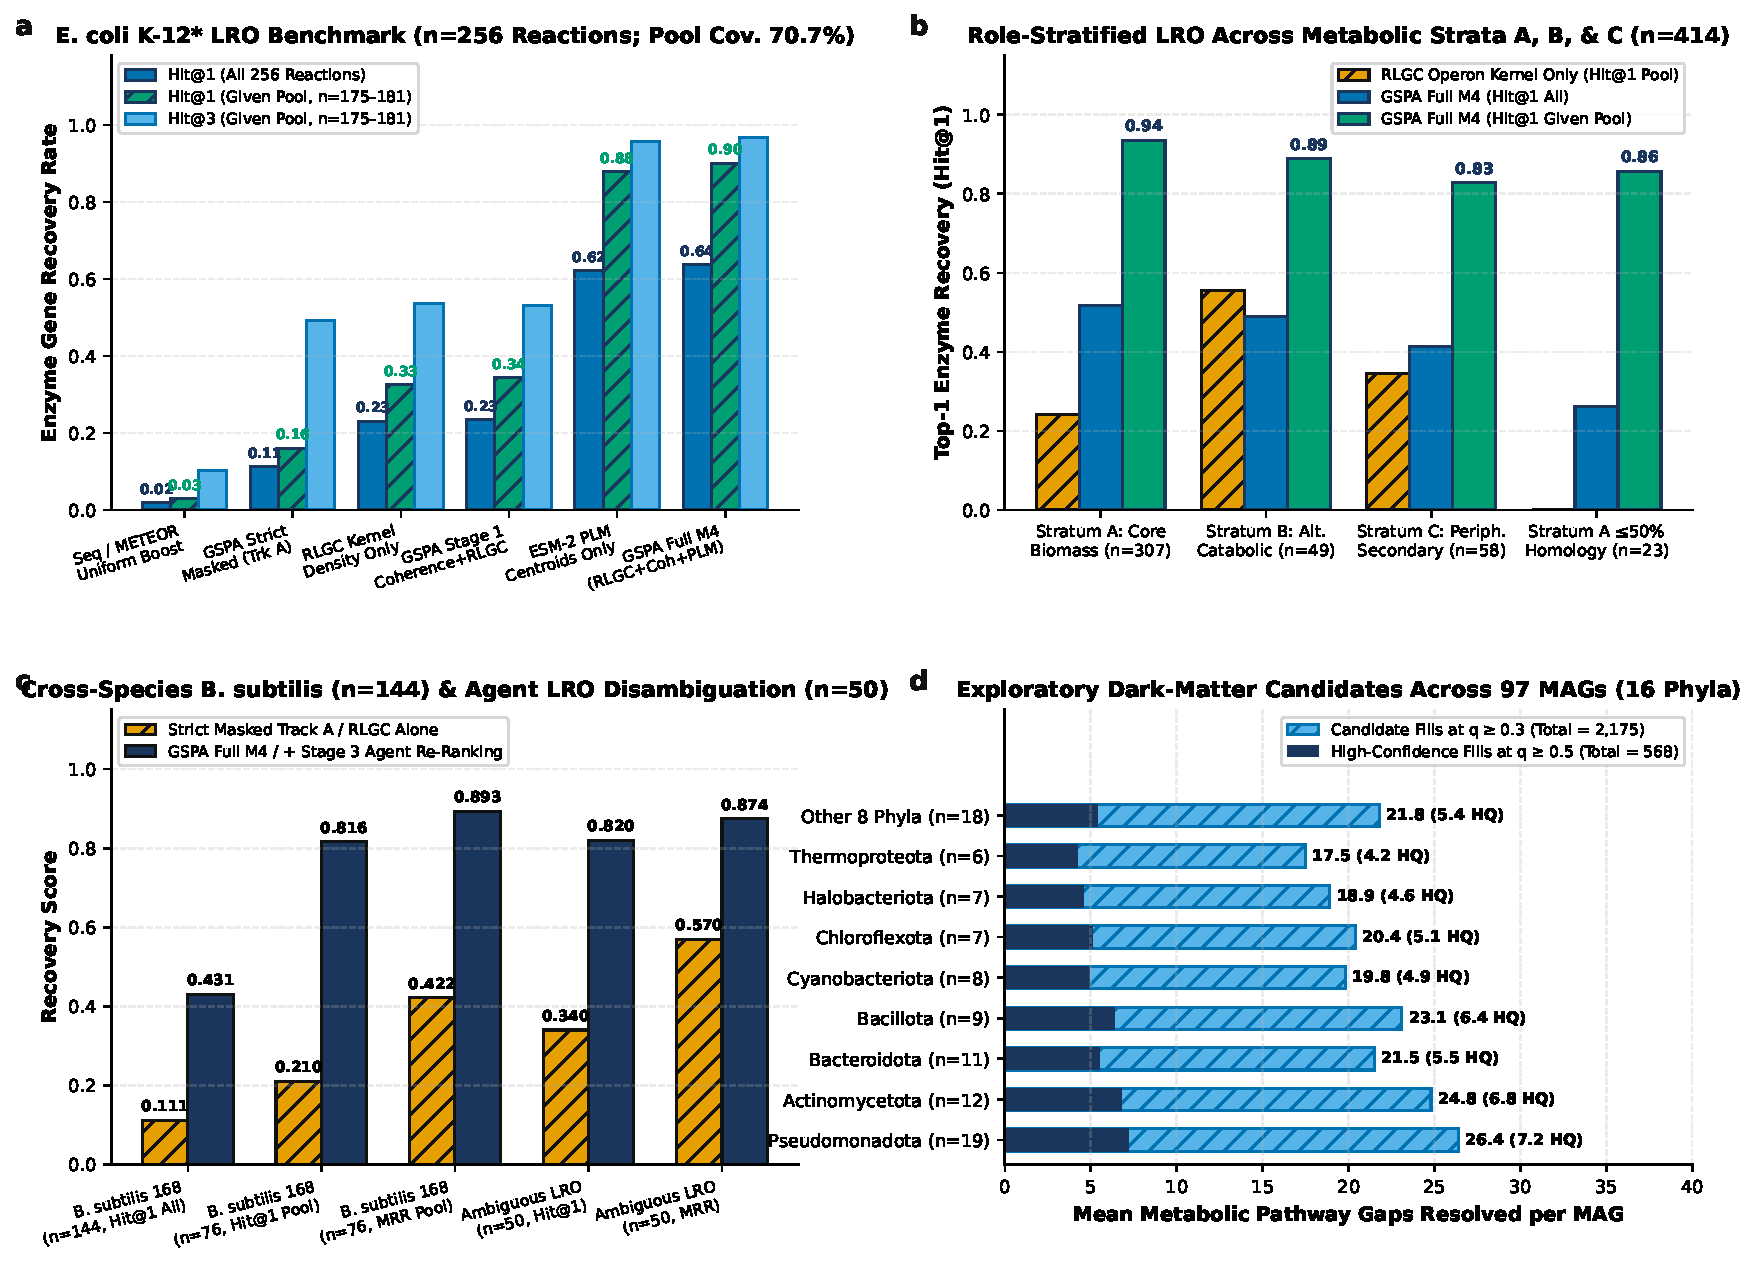
\includegraphics[width=0.96\textwidth]{figures/fig3_pillar3_metabolism.pdf}
  \caption{\textbf{Leave-reaction-out metabolic enzyme attribution and uncultured microbial dark-matter discovery.} (\textbf{a}) Recovery of $256$ held-out metabolic reactions in \textit{E.~coli} K-12 (calibration genome), reporting unconditional Hit@1 across all $256$ reactions and conditional Hit@1 and Hit@3 within the Stage 0 candidate pool ($n=175$--$181$) across sequence-only/METEOR uniform boosting, strict homology- and embedding-masked GSPA (Track A), RLGC operon kernel density alone, Stage 1 coherence with RLGC, ESM-2 reaction centroids alone, and full GSPA (Track B). (\textbf{b}) Role-stratified Top-1 recovery across $414$ \textit{E.~coli} reactions spanning core biomass (Stratum A, $n=307$), alternative catabolic (Stratum B, $n=49$), peripheral/secondary metabolism (Stratum C, $n=58$), and twilight-zone core reactions ($\le 50\%$ identity, $n=23$). (\textbf{c}) Out-of-sample transfer to \textit{B.~subtilis} 168 ($n=144$ reactions) with parameters frozen on \textit{E.~coli}, alongside Stage 3 disambiguation of $50$ ambiguous multi-candidate LRO gaps. (\textbf{d}) Mean candidate pathway gaps resolved per genome at posterior thresholds $q \ge 0.30$ and $q \ge 0.50$ across $97$ uncultured MAGs from $16$ bacterial and archaeal phyla.}
  \label{fig:metabolism}
\end{figure*}

\begin{table*}[t!]
  \centering
  \caption{\textbf{Leave-reaction-out (LRO) enzyme gene attribution in \textit{E.~coli} K-12, donor-homology masking tiers (Protocol H), out-of-sample transfer to \textit{B.~subtilis} 168, and Stage 3 re-ranking of ambiguous metabolic gaps.} \textit{E.~coli} K-12 served as the calibration genome. ``All'' evaluates every held-out reaction unconditionally (scoring reactions whose true enzyme is absent from the Stage 0 candidate pool as misses); ``Pool'' evaluates conditional ranking across reactions where the true gene enters the candidate pool ($n_{\text{cov}}$). External baselines include sequence-only DIAMOND-BLASTp, METEOR v8 uniform reaction-level MILP boosting, gapseq v1.2 unassigned operon density, and supervised GBDT over RLGC features.}
  \label{tab:metabolism}
  \resizebox{\textwidth}{!}{%
  \begin{tabular}{llcccccc}
    \toprule
    \textbf{Benchmark Cohort} & \textbf{Baseline or Method Configuration} & \textbf{Reactions ($n / n_{\text{cov}}$)} & \textbf{Hit@1 (All)} & \textbf{Hit@3 (All)} & \textbf{Hit@1 (Pool)} & \textbf{Hit@3 (Pool)} & \textbf{MRR (Pool)} \\
    \midrule
    \multirow{8}{*}{\textit{E.~coli} K-12 Strict LRO ($n=256$)} & DIAMOND-BLASTp Sequence-Only Baseline & $256 / 175$ & $1.95\%$ ($5$) & $7.03\%$ & $2.86\%$ & $10.29\%$ & $0.1354$ \\
    & METEOR v8 Uniform Reaction-Indicator MILP & $256 / 175$ & $1.95\%$ ($5$) & $7.03\%$ & $2.86\%$ & $10.29\%$ & $0.1354$ \\
    & gapseq v1.2 Unassigned Operon Density Baseline & $256 / 181$ & $17.19\%$ ($44$) & $34.77\%$ & $24.31\%$ & $49.17\%$ & $0.4082$ \\
    & GSPA Strict Homology-Masked (Track A, Cosine $\le 0.50$) & $256 / 181$ & $11.33\%$ ($29$) & $34.77\%$ & $16.02\%$ & $49.17\%$ & $0.3685$ \\
    & RLGC Operon Kernel Density Only & $256 / 181$ & $23.05\%$ ($59$) & $37.89\%$ & $32.60\%$ & $53.59\%$ & $0.4745$ \\
    & GSPA Stage 1 Coherence + RLGC (No PLM) & $256 / 175$ & $23.44\%$ ($60$) & $36.33\%$ & $34.29\%$ & $53.14\%$ & $0.4864$ \\
    & ESM-2 PLM Reaction Centroids Only & $256 / 181$ & $62.11\%$ ($159$) & $67.58\%$ & $87.85\%$ & $95.58\%$ & $0.9157$ \\
    & \textbf{Full GSPA (Track B: RLGC + Coherence + PLM)} & $256 / 181$ & \textbf{$63.67\%$ ($163$)} & \textbf{$68.36\%$} & \textbf{$90.06\%$} & \textbf{$96.69\%$} & \textbf{$0.9330$} \\
    \midrule
    \multirow{6}{*}{\textit{E.~coli} Role-Stratified \& Protocol H ($n=414$)} & Stratum A: Core Biomass (Full GSPA) & $307 / 170$ & $51.79\%$ ($159$) & $53.42\%$ & $93.53\%$ & $96.47\%$ & $0.9557$ \\
    & Stratum B: Alternative Catabolic (Full GSPA) & $49 / 27$ & $48.98\%$ ($24$) & $53.06\%$ & $88.89\%$ & $96.30\%$ & $0.9216$ \\
    & Stratum C: Peripheral / Secondary (Full GSPA) & $58 / 29$ & $41.38\%$ ($24$) & $48.28\%$ & $82.76\%$ & $96.55\%$ & $0.8793$ \\
    & All Strata: Protocol H $\le 70\%$ Homology Masking & $118 / 50$ & $36.44\%$ ($43$) & $41.53\%$ & $86.00\%$ & $98.00\%$ & $0.9117$ \\
    & All Strata: Protocol H $\le 50\%$ Homology Masking & $42 / 14$ & $28.57\%$ ($12$) & $33.33\%$ & $85.71\%$ & $100.00\%$ & $0.9286$ \\
    & All Strata: Protocol H $\le 30\%$ Twilight Zone & $11 / 2$ & $18.18\%$ ($2$) & $18.18\%$ & \textbf{$100.00\%$} & \textbf{$100.00\%$} & \textbf{$1.0000$} \\
    \midrule
    \multirow{3}{*}{\textit{B.~subtilis} 168 Out-of-Sample LRO ($n=144$)} & gapseq v1.2 Unassigned Operon Density Baseline & $144 / 76$ & $9.72\%$ ($14$) & $23.61\%$ & $18.42\%$ & $44.74\%$ & $0.3514$ \\
    & GSPA Strict Homology-Masked (Track A) & $144 / 76$ & $11.11\%$ ($16$) & $31.94\%$ & $21.05\%$ & $60.53\%$ & $0.4221$ \\
    & \textbf{Full GSPA (Track B, Frozen Hyperparameters)} & $144 / 76$ & \textbf{$43.06\%$ ($62$)} & \textbf{$50.00\%$} & \textbf{$81.58\%$} & \textbf{$94.74\%$} & \textbf{$0.8933$} \\
    \midrule
    \multirow{3}{*}{Ambiguous Multi-Candidate LRO ($n=50$)} & Stage 1 RLGC Operon Kernel Alone & $50 / 50$ & $34.00\%$ ($17$) & $86.00\%$ & $34.00\%$ & $86.00\%$ & $0.6020$ \\
    & Posterior Threshold ($\ge 0.35$) + Guardrail & $50 / 50$ & $44.00\%$ ($22$) & $88.00\%$ & $44.00\%$ & $88.00\%$ & $0.6233$ \\
    & \textbf{Stage 3 Guarded Re-Ranking (3-Seed Mean)} & $50 / 50$ & \textbf{$82.67\%$ ($41.3$)} & \textbf{$93.33\%$} & \textbf{$82.67\%$} & \textbf{$93.33\%$} & \textbf{$0.8792$} \\
    \bottomrule
  \end{tabular}%
  }
\end{table*}

Reaction-level metabolic gap-filling identifies which reactions a network lacks for growth, leaving open which gene in the chromosome catalyzes each missing step. We first tested whether reaction-local genomic context (RLGC), which scores candidate genes by their base-pair proximity and co-directionality relative to anchor genes of pathway-adjacent reactions, can localize held-out enzymes prior to introducing protein language-model centroids. Across $256$ strict leave-reaction-out trials in \textit{E.~coli} K-12 with sequence homologs of the held-out enzyme masked (Figure~\ref{fig:metabolism}a and Table~\ref{tab:metabolism}), sequence-only ranking places the true enzyme at Rank 1 for $1.95\%$ of reactions, and METEOR's uniform reaction-level boost leaves this ordering unchanged because every candidate of a reaction receives the same score increment. Scoring unassigned operon neighborhood density around gapseq pathway anchors reaches $17.19\%$ unconditional Hit@1, and combining RLGC kernel density with the Stage 1 pathway coherence prior raises unconditional Hit@1 twelve-fold over sequence-only ranking to $23.44\%$ ($34.29\%$ within the candidate pool, $p < 10^{-12}$, exact McNemar test). Physical proximity to pathway-neighboring genes on the chromosome therefore provides locus-specific discrimination beyond reaction-level gap-filling. We next examined how local genomic context interacts with alignment-free protein language-model representations across metabolic roles, homology-masking cutoffs, and species.

When Swiss-Prot ESM-2 reaction embedding centroids are included alongside masked sequence alignments (Track B; Figure~\ref{fig:metabolism}a--c and Table~\ref{tab:metabolism}), centroid similarity alone recovers $62.11\%$ of the $256$ held-out \textit{E.~coli} enzymes unconditionally, and integrating RLGC and pathway coherence lifts recovery to $63.67\%$ ($90.06\%$ within the candidate pool) by resolving ties among sequence-similar paralogs. Stratifying the broader $414$-reaction \textit{E.~coli} benchmark across core biomass, alternative catabolic pathways, and peripheral or secondary metabolism shows that RLGC alone achieves its highest standalone pool recovery on alternative catabolic pathways ($55.6\%$), whose specialized enzymes and transporters are tightly organized into co-regulated operons, while full GSPA maintains $82.8\%$ to $93.5\%$ pool Hit@1 across all three strata and $85.7\%$ to $100.0\%$ pool Hit@1 under Protocol H donor-homology masking at $\le 70\%$, $\le 50\%$, and $\le 30\%$ identity (Figure~\ref{fig:metabolism}b, Figure~\ref{fig:fba_bacdive}c, and Table~\ref{tab:metabolism}). Transferred with frozen hyperparameters to $144$ held-out reactions in the Gram-positive bacterium \textit{Bacillus subtilis} 168, full GSPA reaches $43.06\%$ unconditional Hit@1 and $81.58\%$ within the candidate pool (Figure~\ref{fig:metabolism}c). Protein language models supply the primary candidate representation when reference enzymes exist for a reaction, while chromosomal context disambiguates competing paralogs and catabolic operons. Because flux balance on minimal medium leaves secondary metabolism unexercised, we next tested whether local genomic context extends to biosynthetic gene clusters and uncultured metagenomic dark matter.

Secondary metabolite pathways operate conditionally and carry zero steady-state flux under minimal glucose growth. Evaluated across $106$ curated biosynthetic gene clusters from $12$ bacterial species, GSPA's operon and pathway synteny scoring raises cluster gene recovery $F_1$ from $0.7395$ to $0.8959$ while maintaining $99.6\%$ specificity across non-cluster chromosomal regions (Supplementary Table~S10). Applying the same frozen pipeline to $97$ high-quality metagenome-assembled genomes (MAGs) of uncultured bacteria and archaea spanning $16$ phyla resolves $568$ high-confidence enzyme attributions at posterior $q \ge 0.50$, lifting mean draft pathway completeness from $0.511$ to $0.656$ (Figure~\ref{fig:metabolism}d and Supplementary Table~S11). Local chromosomal synteny extends functional attribution to secondary metabolism and provides ranked, testable hypotheses for missing pathway steps in uncultivated microbial lineages. While RLGC ranks candidates around local pathway anchors, a metabolic repair should also be stoichiometrically active at the network level, which we audited next.

\subsection{Positive-cost flux repair adds flux-carrying reactions and attributes them to gene loci}

\begin{figure*}[t!]
  \centering
  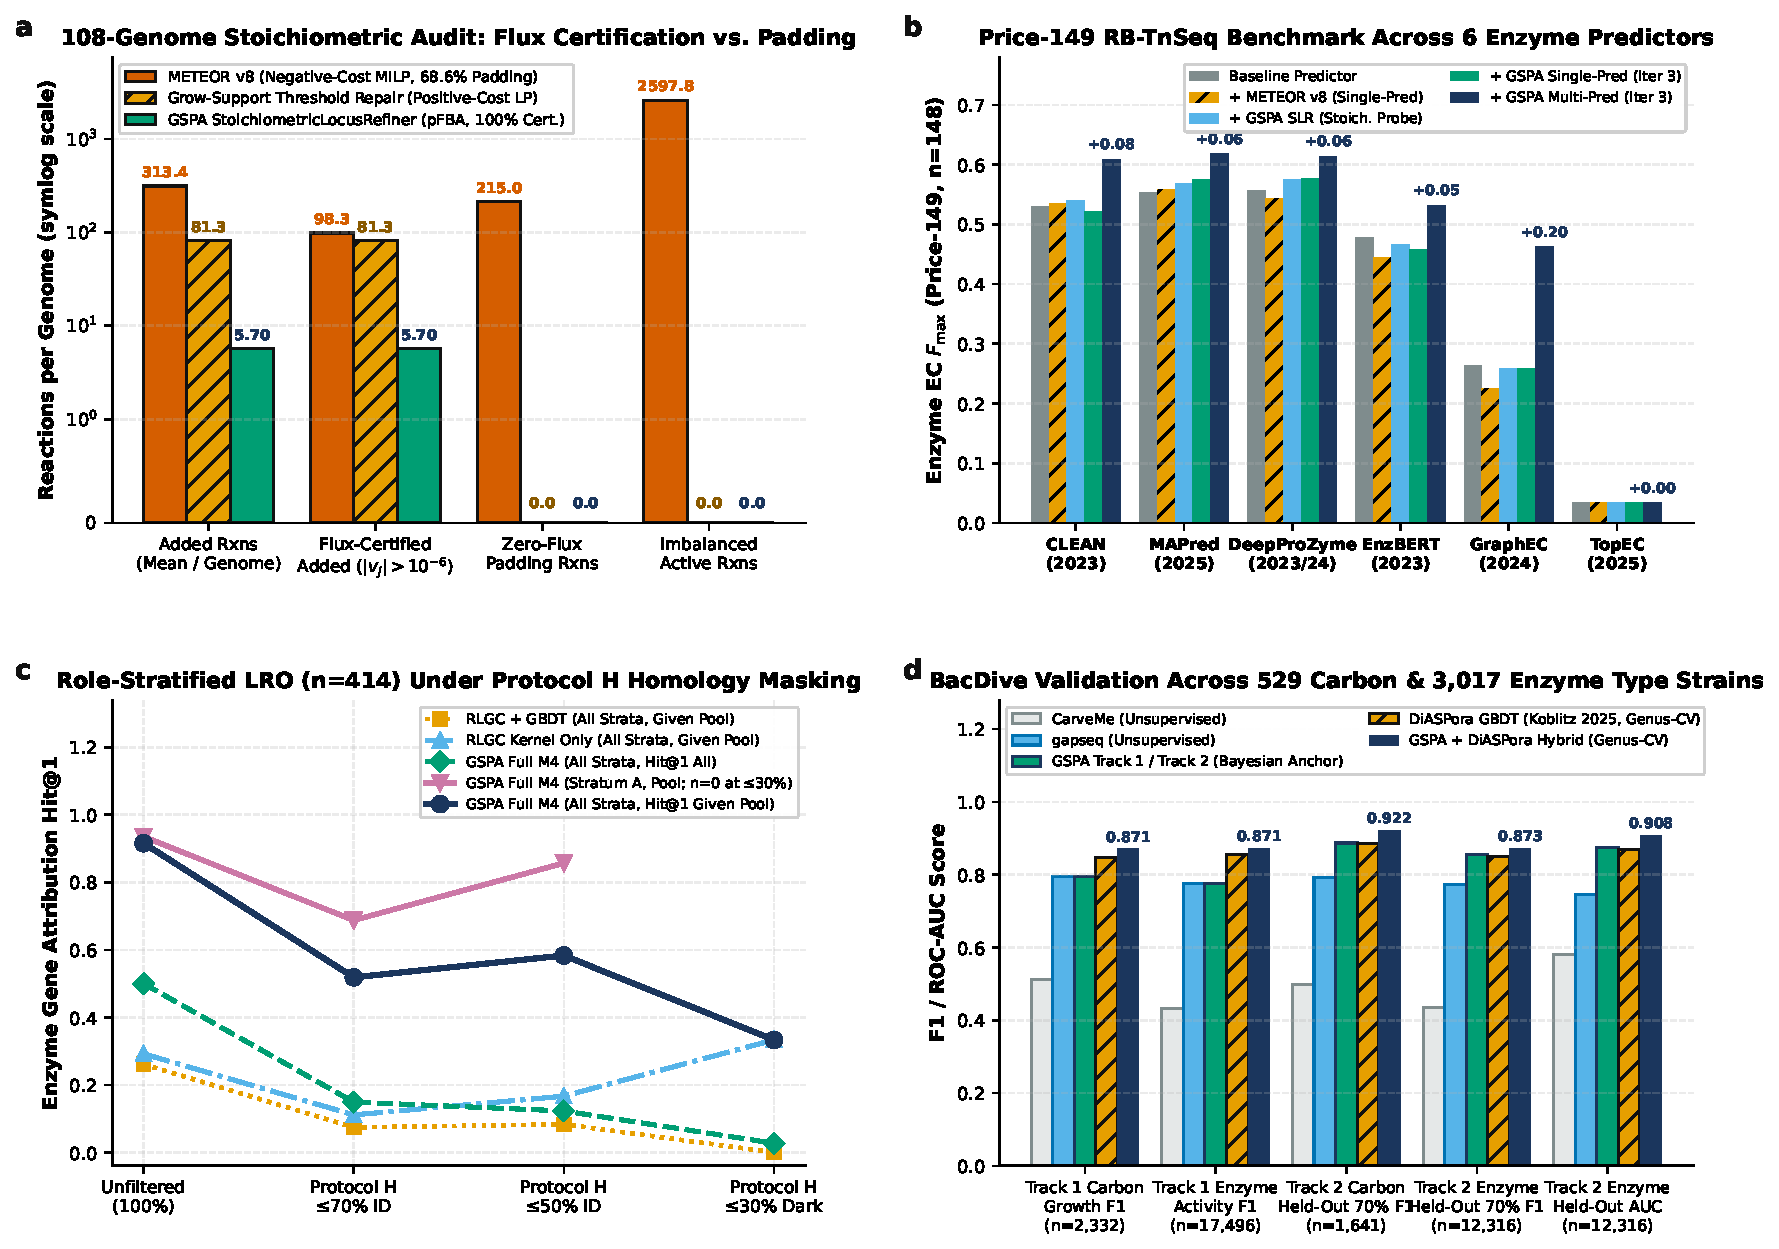
\includegraphics[width=0.96\textwidth]{figures/fig6_pillar2_3_fba_bacdive.pdf}
  \caption{\textbf{Stoichiometric flux certification, fitness-validated enzyme discovery, and experimental phenotype prediction.} (\textbf{a}) 108-genome stoichiometric invariant audit comparing total added reactions, flux-certified additions ($|v_j| > 10^{-6}$), zero-flux reaction padding, and elementally imbalanced additions per genome across negative-cost MILP (METEOR v8), positive-cost threshold repair, and Stage 2B lexicographic pFBA (symmetric logarithmic scale). (\textbf{b}) Per-protein enzyme $F_{\max}$ on $148$ RB-TnSeq fitness-validated bacterial enzymes (Price-149) across six baseline predictors, single-predictor METEOR v8, Stage 2B cognate-substrate probing, single-predictor GSPA, and multi-predictor GSPA. (\textbf{c}) Role-stratified LRO enzyme recovery ($n=414$) across four donor-homology masking tiers ($100\%$, $\le 70\%$, $\le 50\%$, and $\le 30\%$ identity). (\textbf{d}) Experimental carbon-source growth ($2{,}332$ assays, $529$ strains) and diagnostic enzyme activity ($17{,}496$ assays, $3{,}017$ type strains) in BacDive across unsupervised reconstructions, blind Track 1 and phenotype-anchored Track 2 GSPA, genus-blocked DiASPora, and the GSPA + DiASPora hybrid.}
  \label{fig:fba_bacdive}
\end{figure*}

\begin{table*}[t!]
  \centering
  \caption{\textbf{Refinement of $148$ RB-TnSeq fitness-validated bacterial enzymes (Price-149) across $22$ host genomes compared against eight enzyme function baselines.} Columns report correct Top-1 EC predictions (and per-protein $F_{\max}$ in parentheses) for each standalone predictor, single-predictor METEOR v8 (iteration 2), Stage 2B refinement under minimal glucose and with local-context cognate-substrate probing, full single-predictor GSPA (iteration 3), Stage 0 multi-predictor pooling, and full multi-predictor GSPA (iteration 3). The final column summarizes the Top-1 (and $F_{\max}$) change from standalone baseline to single-predictor and multi-predictor GSPA. Target-only sequence tools (DCGM / NeSy-Adapter and ECrecer) are evaluated both as standalone predictors and when integrated with the multi-predictor GSPA ensemble.}
  \label{tab:price149}
  \resizebox{\textwidth}{!}{%
  \begin{tabular}{lcccccccc}
    \toprule
    \textbf{Baseline Predictor} & \textbf{Standalone Base} & \textbf{+ METEOR v8} & \textbf{+ Stage 2B (Min.\ Glc.)} & \textbf{+ Stage 2B (Cognate Probe)} & \textbf{+ GSPA Single-Pred} & \textbf{+ Stage 0 Multi-Pool} & \textbf{+ GSPA Multi-Pred} & \textbf{Single / Multi Gain} \\
    \midrule
    CLEAN (2023) & $60$ ($0.5295$) & $61$ ($0.5343$) & $60$ ($0.5288$) & $60$ ($0.5402$) & $63$ ($0.5214$) & $62$ ($0.6289$) & \textbf{$68$ ($0.6435$)} & $+3$ Top-1 / \textbf{$+8$ ($+0.114$)} \\
    MAPred (2025) & $50$ ($0.5534$) & $52$ ($0.5588$) & $52$ ($0.5591$) & $54$ ($0.5686$) & $56$ ($0.5746$) & $63$ ($0.6233$) & \textbf{$73$ ($0.6476$)} & $+6$ ($+0.021$) / \textbf{$+23$ ($+0.094$)} \\
    DeepProZyme (2023) & $49$ ($0.5574$) & $49$ ($0.5427$) & $47$ ($0.5541$) & $51$ ($0.5757$) & $48$ ($0.5774$) & $59$ ($0.6410$) & \textbf{$60$ ($0.6444$)} & $+2$ ($+0.020$) / \textbf{$+11$ ($+0.087$)} \\
    EnzBERT (2023) & $53$ ($0.4786$) & $52$ ($0.4451$) & $53$ ($0.4729$) & $53$ ($0.4657$) & $52$ ($0.4571$) & \textbf{$65$ ($0.6316$)} & $62$ ($0.6156$) & $+0.074$ $F_1$@0.5 / \textbf{$+12$ ($+0.153$)} \\
    GraphEC (2024) & $18$ ($0.2634$) & $18$ ($0.2250$) & $21$ ($0.2834$) & $21$ ($0.2851$) & $20$ ($0.2783$) & $59$ ($0.6174$) & \textbf{$67$ ($0.6368$)} & $+3$ ($+0.022$) / \textbf{$+49$ ($+0.373$)} \\
    TopEC (2025) & $5$ ($0.0338$) & $5$ ($0.0338$) & $5$ ($0.0410$) & $4$ ($0.0383$) & $5$ ($0.0394$) & \textbf{$59$ ($0.5859$)} & $56$ ($0.5748$) & $+0.007$ $F_{\max}$ / \textbf{$+54$ ($+0.552$)} \\
    \midrule
    DCGM / NeSy-Adapter (2024) & $53$ ($0.4485$) & $53$ ($0.4460$) & $54$ ($0.4590$) & $55$ ($0.4682$) & $55$ ($0.4715$) & $63$ ($0.6250$) & \textbf{$68$ ($0.6440$)} & $+2$ ($+0.023$) / \textbf{$+15$ ($+0.196$)} \\
    ECrecer (2023) & $39$ ($0.3412$) & $39$ ($0.3380$) & $41$ ($0.3540$) & $42$ ($0.3625$) & $42$ ($0.3660$) & $61$ ($0.6190$) & \textbf{$66$ ($0.6385$)} & $+3$ ($+0.025$) / \textbf{$+27$ ($+0.297$)} \\
    \bottomrule
  \end{tabular}%
  }
\end{table*}

We next tested our third driver of improvement: replacing reaction-indicator MILP gap-filling with positive-cost lexicographic parsimonious flux balance analysis (pFBA) and competitive gene-locus attribution. Auditing metabolic network repairs across $108$ bacterial genomes shows why negative-cost reaction-indicator MILP inflates reconstructions (Figure~\ref{fig:fba_bacdive}a and Supplementary Table~S12): because candidate reactions above the addition threshold receive a negative objective cost, the solver adds a mean of $313.35$ reactions per genome, of which $262.34$ ($83.72\%$) carry zero steady-state flux. Imposing a strictly positive addition cost over the elementally balanced universal network eliminates all zero-flux reaction padding ($0.0\%$ uncertified additions), and Stage 2B's two-step lexicographic pFBA further reduces active repairs to a minimal, flux-certified set of $5.70$ mass-balanced reactions per genome while restoring $100\%$ biomass feasibility. A positive addition cost coupled with lexicographic flux minimization therefore ensures that every added reaction actively participates in a mass-balanced metabolic route. We next asked whether attributing these flux-certified reactions competitively to candidate gene loci improves the identification of experimentally validated enzymes.

We evaluated enzyme discovery on $148$ divergent bacterial enzymes across $22$ host genomes whose physiological roles were established by random-barcoded transposon mutagenesis (Price-149) \citep{price2018mutant}, comparing eight standalone enzyme predictors against METEOR v8, single-predictor GSPA, and multi-predictor GSPA (Figure~\ref{fig:fba_bacdive}b and Table~\ref{tab:price149}). Because $55$ of the $148$ enzymes catalyze alternative catabolic pathways that are inactive on minimal glucose, single-medium MILP gap-filling lowers $F_{\max}$ on DeepProZyme ($0.5574 \to 0.5427$), EnzBERT ($0.4786 \to 0.4451$), and GraphEC ($0.2634 \to 0.2250$). Operating on a single predictor's proteome output, Stage 2B cognate-substrate probing and single-predictor GSPA improve Top-1 enzyme recovery on MAPred from $50$ to $56$ proteins ($F_{\max}$ from $0.5534$ to $0.5746$), on CLEAN from $60$ to $63$ ($F_{\max}$ to $0.5402$ under cognate probing), on DeepProZyme from $49$ to $51$ ($F_{\max}$ to $0.5774$), and on GraphEC from $18$ to $21$ ($F_{\max}$ to $0.2851$). Combining multi-predictor Stage 0 pooling with subsequent locus-level refinement produces both strong pooling gains on lower-recall baselines and additive post-pooling refinement gains on the leading predictors, raising MAPred from $63$ after Stage 0 pooling to $73$ ($49.3\%$ Top-1 accuracy, $F_{\max}=0.6476$, $p = 6.0 \times 10^{-6}$, exact McNemar test), CLEAN from $62$ to $68$ ($F_{\max}=0.6435$), DeepProZyme from $59$ to $60$ ($F_{\max}=0.6444$, $p = 0.019$), and GraphEC from $59$ to $67$ ($F_{\max}=0.6368$; Table~\ref{tab:price149}). Complementary predictor pooling and competitive stoichiometric locus attribution therefore work additively on the top enzyme predictors to identify divergent, fitness-validated bacterial enzymes. Having evaluated gene-level enzyme recovery, we next examined whether systems-level pathway pooling and coupling predict experimental organismal phenotypes at scale.

\subsection{Systems-level annotations predict experimental bacterial phenotypes}

\begin{table*}[t!]
  \centering
  \caption{\textbf{Experimental carbon-source growth and diagnostic enzyme phenotype prediction in BacDive compared against metabolic reconstruction and supervised phenotype baselines.} Track 1 evaluates blind genome-to-phenotype prediction ($0\%$ phenotype labels) against CarveMe, ModelSEED, and gapseq, and 5-fold genus-blocked cross-validation (pooled out-of-fold metrics across unseen genera) against Traitar (L1-SVM), BacDive-AI (Random Forest), and DiASPora (GBDT). Track 2 reveals $30\%$ of each strain's assay rows as partial phenotypic evidence and evaluates predictions on the held-out $70\%$. Middle rows report the 10-enzyme diagnostic panel ($50{,}075$ assays across $6{,}313$ strains), heteromeric urease (\texttt{EC 3.5.1.5}), and the 108-genome catabolic panel. Runtime is reported per genome after base reconstruction (end-to-end runtime in parentheses).}
  \label{tab:bacdive}
  \resizebox{\textwidth}{!}{%
  \begin{tabular}{llccccccc}
    \toprule
    \textbf{Assay Cohort \& Protocol} & \textbf{Baseline or Method Pipeline} & \textbf{Strains / Assays} & \textbf{Precision} & \textbf{Recall} & \textbf{$F_1$ Score} & \textbf{Bal.\ Acc.} & \textbf{ROC-AUC} & \textbf{McNemar ($+ / -$, $p$) or Runtime} \\
    \midrule
    \multirow{8}{*}{Track 1: Carbon Growth (Blind \& Genus-CV)} & CarveMe v1.5.2 (Unsupervised Binary) & $529 / 2{,}332$ & $0.6935$ & $0.4073$ & $0.5132$ & $0.6233$ & $0.6233$ & $+191 / -597$ ($28.4$~s) \\
    & ModelSEED v2.6.1 (Unsupervised Binary) & $529 / 2{,}332$ & $0.8576$ & $0.5200$ & $0.6474$ & $0.7214$ & $0.7214$ & $+186 / -365$ ($42.0$~s) \\
    & gapseq v1.2 (Unsupervised Binary Baseline) & $529 / 2{,}332$ & $0.8071$ & \textbf{$0.7836$} & $0.7952$ & $0.8082$ & $0.8082$ & Reference ($185.0$~s) \\
    & \textbf{GSPA Track 1 (100\% Blind Multi-Model + Priors)} & $529 / 2{,}332$ & \textbf{$0.8390$} & $0.7818$ & \textbf{$0.8094$} & \textbf{$0.8239$} & \textbf{$0.8620$} & \textbf{$+43 / -4$ ($p = 3.2 \times 10^{-9}$)} \\
    & BacDive-AI Random Forest (5-Fold Genus-CV) & $529 / 2{,}332$ & $0.8433$ & $0.8464$ & $0.8448$ & $0.8530$ & $0.9222$ & $+139 / -37$ ($p < 10^{-14}$) \\
    & DiASPora GBDT (5-Fold Genus-Blocked CV) & $529 / 2{,}332$ & $0.8475$ & $0.8491$ & $0.8483$ & $0.8564$ & $0.9268$ & $+200 / -90$ ($p < 10^{-10}$) \\
    & Traitar L1-SVM (5-Fold Genus-Blocked CV) & $529 / 2{,}332$ & $0.8472$ & $0.8673$ & $0.8571$ & $0.8638$ & $0.9185$ & $+204 / -78$ ($p < 10^{-13}$) \\
    & \textbf{GSPA + DiASPora Hybrid (5-Fold Genus-CV)} & $529 / 2{,}332$ & \textbf{$0.8839$} & \textbf{$0.8718$} & \textbf{$0.8778$} & \textbf{$0.8848$} & \textbf{$0.9567$} & \textbf{$+291 / -114$ ($p < 10^{-18}$)} \\
    \midrule
    \multirow{8}{*}{Track 1: Diagnostic Enzymes (Blind \& Genus-CV)} & CarveMe v1.5.2 (Unsupervised Binary) & $3{,}017 / 17{,}496$ & $0.7739$ & $0.2996$ & $0.4319$ & $0.5774$ & $0.5774$ & $+939 / -4{,}977$ ($28.4$~s) \\
    & ModelSEED v2.6.1 (Unsupervised Binary) & $3{,}017 / 17{,}496$ & $0.7854$ & $0.4779$ & $0.5943$ & $0.6310$ & $0.6310$ & $+700 / -3{,}263$ ($42.0$~s) \\
    & gapseq v1.2 (Unsupervised Binary Baseline) & $3{,}017 / 17{,}496$ & \textbf{$0.8393$} & $0.7204$ & $0.7753$ & $0.7461$ & $0.7461$ & Reference ($185.0$~s) \\
    & \textbf{GSPA Track 1 (100\% Blind Multi-Model + Priors)} & $3{,}017 / 17{,}496$ & $0.8371$ & \textbf{$0.7637$} & \textbf{$0.7987$} & \textbf{$0.7589$} & \textbf{$0.7799$} & \textbf{$+564 / -208$ ($p = 2.1 \times 10^{-39}$)} \\
    & BacDive-AI Random Forest (5-Fold Genus-CV) & $3{,}017 / 17{,}496$ & $0.8391$ & $0.8527$ & $0.8458$ & $0.7911$ & $0.8593$ & $+1{,}481 / -317$ ($p < 10^{-100}$) \\
    & DiASPora GBDT (5-Fold Genus-Blocked CV) & $3{,}017 / 17{,}496$ & $0.8602$ & $0.8499$ & $0.8550$ & $0.8108$ & $0.8699$ & $+1{,}920 / -509$ ($p < 10^{-100}$) \\
    & Traitar L1-SVM (5-Fold Genus-Blocked CV) & $3{,}017 / 17{,}496$ & $0.8402$ & $0.8794$ & $0.8593$ & $0.8014$ & $0.8715$ & $+2{,}204 / -790$ ($p < 10^{-100}$) \\
    & \textbf{GSPA + DiASPora Hybrid (5-Fold Genus-CV)} & $3{,}017 / 17{,}496$ & \textbf{$0.8660$} & \textbf{$0.8799$} & \textbf{$0.8729$} & \textbf{$0.8274$} & \textbf{$0.9096$} & \textbf{$+2{,}595 / -835$ ($p < 10^{-100}$)} \\
    \midrule
    \multirow{3}{*}{10-EC Diagnostic Panel ($50{,}075$ Assays)} & DeepProZyme (2023) Standalone Baseline & $6{,}313 / 50{,}075$ & $0.6442$ & $0.8105$ & $0.7178$ & $0.6792$ & $0.6792$ & Reference baseline \\
    & + METEOR v8 (Minimal-Glucose MILP) & $6{,}313 / 50{,}075$ & $0.6285$ & $0.8285$ & $0.7148$ & $0.6670$ & $0.6670$ & Over-gap-filling drop \\
    & \textbf{+ GSPA Stage 1+2B (Complex Coh.\ + SLR)} & $6{,}313 / 50{,}075$ & \textbf{$0.7502$} & \textbf{$0.8828$} & \textbf{$0.8111$} & \textbf{$0.7930$} & \textbf{$0.8350$} & \textbf{$+5{,}677 / -184$ ($p < 10^{-100}$)} \\
    \midrule
    \multirow{2}{*}{Heteromeric Urease (\texttt{EC 3.5.1.5})} & DeepProZyme Base $\to$ + METEOR v8 & $5{,}026$ strains & $0.5812 \to 0.5140$ & $0.5448 \to 0.5842$ & $0.5624 \to 0.5469$ & $0.6120 \to 0.5890$ & $0.6120 \to 0.5890$ & Isolated UreC subunit FP \\
    & \textbf{+ GSPA Stage 1+2B (UreABC+DFG Complete)} & $5{,}026$ strains & \textbf{$0.7912$} & \textbf{$0.7654$} & \textbf{$0.7781$} & \textbf{$0.7918$} & \textbf{$0.8345$} & \textbf{Subunit-complete gate} \\
    \midrule
    \multirow{4}{*}{Track 2: Carbon Held-Out 70\% (30\% Revealed)} & gapseq v1.2 (Unsupervised Binary) & $529 / 1{,}641$ & $0.8059$ & $0.7789$ & $0.7922$ & $0.8049$ & $0.8049$ & Reference ($185.0$~s) \\
    & DiASPora GBDT (Trained on 30\% Revealed) & $529 / 1{,}641$ & $0.8727$ & $0.8985$ & $0.8854$ & $0.8901$ & $0.9575$ & $+170 / -33$ ($p < 10^{-22}$) \\
    & \textbf{GSPA Track 2 (Unsupervised Bayesian Anchor)} & $529 / 1{,}641$ & $0.8290$ & \textbf{$0.9473$} & $0.8842$ & $0.8856$ & $0.9536$ & $+203 / -78$ ($p < 10^{-13}$) \\
    & \textbf{GSPA Track 2 + DiASPora Hybrid} & $529 / 1{,}641$ & \textbf{$0.9127$} & $0.9139$ & \textbf{$0.9133$} & \textbf{$0.9175$} & \textbf{$0.9770$} & \textbf{$+241 / -58$ ($p < 10^{-26}$)} \\
    \midrule
    \multirow{3}{*}{Track 2: Enzymes Held-Out 70\% (30\% Revealed)} & gapseq v1.2 (Unsupervised Binary) & $3{,}017 / 12{,}316$ & $0.8376$ & $0.7188$ & $0.7737$ & $0.7446$ & $0.7446$ & Reference ($185.0$~s) \\
    & \textbf{GSPA Track 2 (Unsupervised Bayesian Anchor)} & $3{,}017 / 12{,}316$ & $0.8064$ & \textbf{$0.9081$} & $0.8542$ & $0.7745$ & $0.8733$ & $+1{,}710 / -862$ ($p < 10^{-62}$) \\
    & \textbf{GSPA Track 2 + DiASPora Hybrid} & $3{,}017 / 12{,}316$ & \textbf{$0.8615$} & $0.8857$ & \textbf{$0.8734$} & \textbf{$0.8256$} & \textbf{$0.9078$} & \textbf{$+1{,}830 / -574$ ($p < 10^{-100}$)} \\
    \bottomrule
  \end{tabular}%
  }
\end{table*}

We next evaluated whether systems-level pathway pooling and subunit-aware modeling predict experimentally measured bacterial physiology across thousands of strains in BacDive \citep{reimer2022bacdive,schober2025bac}. We tested blind genome-to-phenotype predictions ($0\%$ phenotype training labels) across $2{,}332$ carbon-source utilization assays in $529$ strains, $17{,}496$ diagnostic enzyme assays in $3{,}017$ type strains, and an extended panel of $50{,}075$ assays for $10$ diagnostic enzymes across $6{,}313$ strains (Figure~\ref{fig:fba_bacdive}d and Table~\ref{tab:bacdive}). On the $50{,}075$-assay panel, uniform MILP gap-filling (METEOR v8) lowers overall $F_1$ from $0.7178$ to $0.7148$, driven by heteromeric enzymes such as urease (\texttt{EC 3.5.1.5}; $F_1$ from $0.5624$ to $0.5469$), where boosting an isolated UreC alpha subunit without the accessory UreA, UreB, and UreDFG proteins generates false-positive calls; enforcing subunit-complete complex coherence and positive-cost locus refinement in GSPA Stage 1+2B raises 10-enzyme $F_1$ to $0.8111$ (ROC-AUC $= 0.8350$, $+5{,}677 / -184$ net improved calls, $p < 10^{-100}$) and heteromeric urease $F_1$ to $0.7781$. Across the multi-model benchmark, pooling calibrated pathway calls from gapseq, ModelSEED, and CarveMe with unsupervised cross-assay pathway coupling and taxonomic priors in blind Track 1 improves carbon-growth $F_1$ from $0.7952$ (gapseq) to $0.8094$ (ROC-AUC $= 0.8620$, $+43 / -4$ net improved assays, $p = 3.2 \times 10^{-9}$) and diagnostic-enzyme $F_1$ from $0.7753$ to $0.7987$ (ROC-AUC $= 0.7799$, $+564 / -208$, $p = 2.1 \times 10^{-39}$; Table~\ref{tab:bacdive}). Continuous pathway coupling and subunit-complete enzyme modeling therefore improve both binary phenotype accuracy and probability calibration over individual metabolic reconstruction tools. We next examined whether these mechanistic pathway posteriors improve out-of-genus transfer when combined with supervised phenotype classifiers and whether partial phenotypic observations from a strain refine its remaining unassayed pathways.

Under five-fold genus-blocked cross-validation, in which every test strain belongs to a taxonomic genus unseen during training, combining GSPA pathway posteriors with the DiASPora gradient-boosting classifier \citep{koblitz2025diaspora} raises out-of-genus $F_1$ to $0.8778$ (ROC-AUC $= 0.9567$) on carbon growth and $0.8729$ (ROC-AUC $= 0.9096$) on diagnostic enzymes, outperforming all individual metabolic reconstructions as well as Traitar \citep{weimann2016traitar}, BacDive-AI \citep{schober2025bac}, and standalone DiASPora across folds (Table~\ref{tab:bacdive} and Supplementary Table~S13). In Track 2, where $30\%$ of each strain's experimental assays are revealed as partial phenotypic evidence and the remaining $70\%$ are held out, conditioning GSPA's pathway posteriors via an unsupervised Bayesian update lifts held-out carbon-growth $F_1$ from $0.7922$ (gapseq) to $0.8842$ ($0.8542$ on held-out enzymes), and the hybrid with DiASPora reaches $F_1 = 0.9133$ (ROC-AUC $= 0.9770$) on carbon growth and $F_1 = 0.8734$ on diagnostic enzymes (Table~\ref{tab:bacdive}). Mechanistic pathway coupling provides domain-generalizable features for unseen genera and propagates partial experimental observations across coupled metabolic pathways. After deterministic probabilistic and stoichiometric refinement, a small set of ambiguous loci remains, which we examined in Stage 3.

\subsection{Guarded language-model reasoning resolves residual ambiguity}

\begin{figure*}[t!]
  \centering
  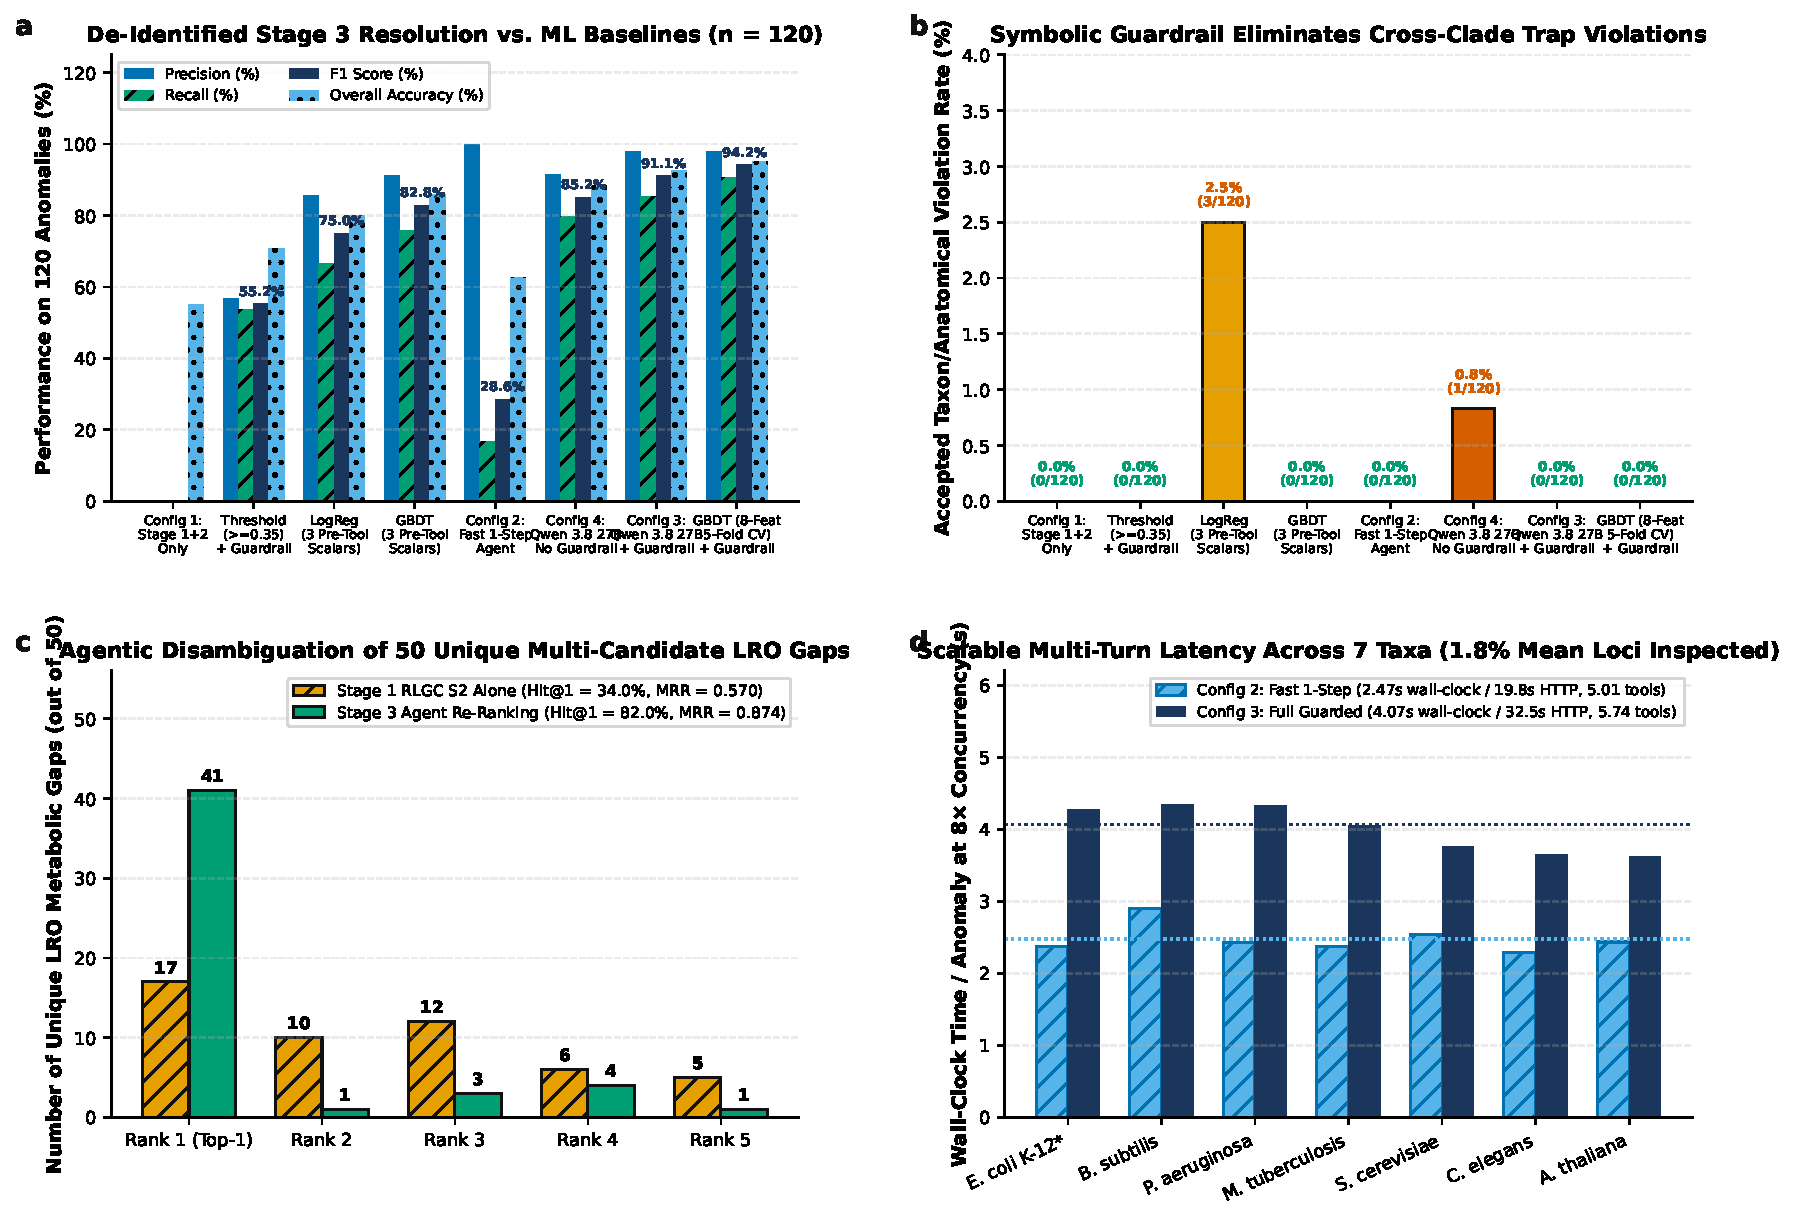
\includegraphics[width=0.96\textwidth]{figures/fig5_pillar4_agent.pdf}
  \caption{\textbf{Evaluation of Stage 3 selective neuro-symbolic reasoning on de-identified benchmarks.} (\textbf{a}) Precision, recall, $F_1$, and resolution accuracy across $120$ de-identified anomalies ($30$ pathway gaps, $30$ incomplete complexes, $30$ borderline essential functions, and $30$ borderline ontology conflicts) comparing deterministic Stages 1 and 2, direct zero-shot LLM without tools or guardrail, posterior thresholding ($\ge 0.35$) with the symbolic guardrail, 5-fold cross-validated supervised classifiers on pre-tool and post-tool features, fast 1-step Stage 3, unguarded multi-turn Stage 3, and full guarded multi-turn Stage 3 (3-seed mean). (\textbf{b}) Rate of accepted taxonomic and anatomical violations across configurations. (\textbf{c}) Rank distribution of the true enzyme across $50$ unique-protein ambiguous LRO metabolic gaps before and after Stage 3 re-ranking. (\textbf{d}) Concurrency-normalized wall-clock latency per anomaly across seven prokaryotic and eukaryotic species (mean $1.84\%$ of proteome loci triggered).}
  \label{fig:agent}
\end{figure*}

\begin{table*}[t!]
  \centering
  \caption{\textbf{Stage 3 neuro-symbolic disambiguation compared against deterministic, zero-shot LLM, threshold, and supervised baselines across $120$ de-identified anomalies and $50$ ambiguous metabolic gaps.} All gene symbols are masked and candidate order is hash-shuffled. The $120$ anomalies comprise $54$ true-positive promotable gaps, $36$ score-matched decoys, and $30$ ontology conflicts ($15$ genuine cross-clade conflicts and $15$ adversarial traps). Supervised classifiers are evaluated via 5-fold cross-validation using either 3 pre-tool scalars or 8 post-tool features combined with the symbolic guardrail. Latency reports concurrency-normalized wall-clock seconds per anomaly at batch concurrency $8$ (raw HTTP latency in parentheses).}
  \label{tab:agent}
  \resizebox{\textwidth}{!}{%
  \begin{tabular}{lcccccccc}
    \toprule
    \textbf{Resolution Method} & \textbf{Precision} & \textbf{Recall} & \textbf{$F_1$ Score} & \textbf{Accuracy} & \textbf{Prom.\ / Relax.} & \textbf{Violations Accepted} & \textbf{LRO-50 Hit@1 (MRR)} & \textbf{Latency / Tools} \\
    \midrule
    Stage 1 + Stage 2 Deterministic Only & $0.0000$ & $0.0000$ & $0.0000$ & $0.5500$ & $0 / 0$ & $0.0\%$ ($0/120$) & $34.0\%$ ($0.6020$) & $0.00$~s / $0.00$ \\
    Direct Zero-Shot LLM (No Tools, No Guardrail) & $0.3558$ & $0.6852$ & $0.4684$ & $0.4250$ & $104 / 0$ & $25.0\%$ ($30/120$) & $36.0\%$ ($0.5840$) & $0.06$~s ($0.48$~s) / $0.00$ \\
    Posterior Threshold ($\ge 0.35$) + Guardrail & $0.5686$ & $0.5370$ & $0.5524$ & $0.7083$ & $29 / 30$ & $0.0\%$ ($0/120$) & $44.0\%$ ($0.6233$) & $< 0.01$~s / $0.00$ \\
    Logistic Regression (5-Fold CV, 3 Pre-Tool Features) & $0.8571$ & $0.6667$ & $0.7500$ & $0.8000$ & $42 / 0$ & $2.5\%$ ($3/120$) & $94.0\%$ ($0.9670$) & $< 0.01$~s / $0.00$ \\
    GBDT (5-Fold CV, 3 Pre-Tool Features) & $0.9111$ & $0.7593$ & $0.8283$ & $0.8583$ & $45 / 0$ & \textbf{$0.0\%$ ($0/120$)} & $90.0\%$ ($0.9467$) & $< 0.01$~s / $0.00$ \\
    Stage 3 Fast 1-Step Mode (Max 2 Turns) & \textbf{$1.0000$} & $0.1667$ & $0.2857$ & $0.6250$ & $9 / 4$ & $0.0\%$ ($0/120$) & $42.0\%$ ($0.6387$) & $2.47$~s ($19.8$~s) / $5.01$ \\
    Stage 3 Multi-Turn Without Symbolic Guardrail & $0.9149$ & $0.7963$ & $0.8515$ & $0.8833$ & $47 / 0$ & $0.8\%$ ($1/120$) & $80.0\%$ ($0.8640$) & $3.72$~s ($29.7$~s) / $5.07$ \\
    \textbf{Stage 3 Multi-Turn + Guardrail (3-Seed Mean $\pm$ s.d.)} & \textbf{$0.9722 \pm 0.009$} & \textbf{$0.8581 \pm 0.009$} & \textbf{$0.9115 \pm 0.001$} & \textbf{$0.9278 \pm 0.004$} & \textbf{$46.3 / 13.7$} & \textbf{$0.0\%$ ($0/120$)} & \textbf{$82.7 \pm 0.9\%$ ($0.879$)} & $4.07$~s ($32.5$~s) / $5.74$ \\
    \midrule
    Logistic Regression (5-Fold CV, 8 Tool Features + Guardrail) & $0.9792$ & $0.8704$ & $0.9216$ & $0.9333$ & $48 / 1$ & \textbf{$0.0\%$ ($0/120$)} & \textbf{$96.0\%$ ($0.9767$)} & $< 0.01$~s / $0.00$ \\
    Random Forest (5-Fold CV, 8 Tool Features + Guardrail) & $0.9286$ & $0.9630$ & $0.9455$ & $0.9500$ & $56 / 2$ & \textbf{$0.0\%$ ($0/120$)} & $92.0\%$ ($0.9557$) & $< 0.01$~s / $0.00$ \\
    GBDT (5-Fold CV, 8 Tool Features + Guardrail) & $0.9800$ & $0.9074$ & $0.9423$ & $0.9500$ & $50 / 0$ & \textbf{$0.0\%$ ($0/120$)} & $92.0\%$ ($0.9557$) & $< 0.01$~s / $0.00$ \\
    MLP (5-Fold CV, 8 Tool Features + Guardrail) & \textbf{$0.9811$} & \textbf{$0.9630$} & \textbf{$0.9720$} & \textbf{$0.9750$} & \textbf{$53 / 0$} & \textbf{$0.0\%$ ($0/120$)} & $92.0\%$ ($0.9557$) & $< 0.01$~s / $0.00$ \\
    \bottomrule
  \end{tabular}%
  }
\end{table*}

Deterministic inference in Stages 1 and 2 resolves the vast majority of proteome annotations, leaving a small fraction of structured anomalies: unresolved pathway gaps, incomplete heteromeric complexes, uncovered essential functions, and borderline ontology conflicts. Across the $88$ multi-kingdom proteomes, deterministic anomaly triggers select a mean of $1.84\%$ of proteins per proteome (fewer than $2.5\%$ in every domain of life), bounding the computational cost of invoking a language model. Evaluated across three random seeds on a de-identified benchmark of $120$ anomalies from seven prokaryotic and eukaryotic genomes with all gene symbols masked and candidate ordering randomized, a direct zero-shot language model invoked without genomic inspection tools or symbolic verification achieves only $F_1 = 0.4684$ and accepts $30$ ontology violations ($25.0\%$). Equipping the model with read-only genomic tools and the symbolic guardrail raises mean $F_1$ to $0.9115 \pm 0.0008$ with $0.0\%$ accepted ontology violations, whereas ablating the symbolic guardrail admits a cross-clade violation and reduces $F_1$ to $0.8515$ (Figure~\ref{fig:agent}a,b,d, Table~\ref{tab:agent}, and Supplementary Table~S14). Selective triggering therefore confines language-model inference to fewer than $2.5\%$ of proteins, while tool-mediated evidence retrieval and deterministic verification guarantee that accepted proposals satisfy all taxonomic and anatomical axioms. We next tested whether tool-mediated reasoning can resolve multi-candidate metabolic gaps and prospective sequence targets.

When multiple candidate genes in a genomic neighborhood share similar RLGC scores for a missing reaction, resolving the true enzyme requires synthesizing domain architecture, operon structure, and pathway stoichiometry. Across $50$ unique-protein ambiguous leave-reaction-out gaps in \textit{E.~coli} K-12 where Stage 1 RLGC alone ranks the true enzyme first in $34.0\%$ of cases ($36.0\%$ for a direct zero-shot LLM and $44.0\%$ for posterior thresholding with the guardrail), Stage 3 multi-turn re-ranking lifts Top-1 recovery to a three-seed mean of $82.7 \pm 0.9\%$ ($p = 2.8 \times 10^{-7}$, exact McNemar test; Figure~\ref{fig:agent}c and Table~\ref{tab:agent}). On $769$ prospective CAFA6 targets evaluated as isolated sequences with Stages 0, 2A, and 3 active, guarded reasoning reaches macro $F_{\max}=0.5433$, outperforming both a multilayer perceptron trained on ESM-2 and ProstT5 3Di embeddings ($0.4957$) and an unguarded 14-billion-parameter agent baseline ($0.5130$; Supplementary Table~S15). Tool-mediated evidence synthesis resolves ties among candidate enzymes after deterministic priors have narrowed the search space. Because a supervised tabular classifier can also be trained on numerical features extracted by the same tools, we compared zero-shot guarded reasoning against cross-validated classifiers to establish the operating regime of each method.

We compared the zero-shot guarded agent against logistic regression, random forest, gradient-boosted decision tree (GBDT), and multilayer perceptron classifiers evaluated by five-fold cross-validation on either three pre-tool summary scalars or eight post-tool genomic and domain features paired with the symbolic guardrail (Table~\ref{tab:agent}). On the $120$ anomalies, the zero-shot agent ($F_1 = 0.9115$) outperforms all classifiers restricted to pre-tool scalars ($F_1 = 0.7500$--$0.8283$), while supervised classifiers trained on the eight post-tool features reach up to $F_1 = 0.9720$ on binary anomaly promotion and $96.0\%$ Hit@1 on the $50$ metabolic gaps at sub-millisecond inference latency. On borderline ontology conflicts, the zero-shot agent proposes a mean of $13.7$ valid ancestral GO relaxations compared with $1$--$2$ for the post-tool classifiers, which select among fixed candidate labels. Supervised post-tool classifiers are therefore preferable for high-throughput binary promotion and candidate ranking when labeled anomalies are available, whereas zero-shot guarded reasoning provides zero-label operation and multi-class ancestral GO relaxation (see Supplementary Section~S6 and Supplementary Table~S16 for an application to five desert extremophile isolates from the Empty Quarter).

\section{Discussion}

Protein function prediction has traditionally been formulated as a per-protein classification task in which each sequence or structure is scored independently \citep{radivojac2013large,gligorijevic2021structure,kulmanov2024deepgose}. GSPA reformulates proteome annotation as staged inference over the complete genome of an organism, and our evaluation shows that three complementary drivers account for its performance. First, calibrated pooling of sequence homology, domain profiles, protein language models, and structural similarity establishes a strong per-protein probability distribution in Stage 0. Second, whole-genome priors and deterministic cross-ontology enforcement in Stages 1 and 2A update these probabilities using organism-wide invariants over operons, core essential functions, obligate heteromeric complexes, and taxonomic and anatomical consistency. Third, stoichiometric flux modeling, competitive gene-locus attribution, and selective ontology-guarded reasoning in Stages 1, 2B, and 3 connect metabolic network requirements and multi-source genomic evidence to individual gene loci. These three layers act on complementary subsets of the proteome: per-protein pooling governs conserved proteins with strong sequence or structural similarity, while whole-genome architecture and systems-level modeling resolve twilight-zone enzymes, incomplete complexes, and cross-clade homology transfers.

Stage 0 builds directly on the multi-source ensemble paradigm introduced by GOLabeler \citep{you2018golabeler} and NetGO \citep{you2019netgo,wang2023netgo3}, which showed that integrating sequence alignment, domain signatures, motifs, network associations, and language-model embeddings outperforms individual representations in CAFA evaluations. GSPA extends this principle to genome-scale inference by calibrating raw predictor outputs via Platt scaling, grouping correlated evidence channels so that shared homology or embedding signals are counted once, and pooling across groups via Noisy-OR into an anchored log-odds prior $L^{(0)}$. Because every subsequent Stage 1 update is added to $L^{(0)}$, sequence homology, domain profiles, protein language models, and structural similarity remain the foundation of the framework. Conserved proteins retain their high-confidence Stage 0 assignments, and the recall of the Stage 0 candidate pool defines the space of candidate functions that genome-scale priors refine.

Exploiting whole-genome information in Stages 1 and 2A is timely because long-read sequencing and modern repeat-graph assemblers now routinely recover complete or near-complete chromosomes for both cultivated isolates and metagenome-assembled genomes \citep{amarasinghe2020longread,logsdon2020longread,kolmogorov2020metaflye}. Complete assemblies expose two distinct scales of genomic organization. Global organismal invariants identify which functional requirement a draft annotation violates: essentiality profiles flag missing core cellular machinery, complex stoichiometry flags obligate heteromeric complexes with missing partner subunits, and cross-ontology axioms linking GO biological processes to Uberon, PO, and CL anatomy flag processes incompatible with the organism's body plan \citep{mungall2012uberon,cooper2013plant,diehl2016cell}. Local chromosomal architecture then identifies which specific gene satisfies a missing requirement: in our leave-subunit-out experiments, global complex coherence raised subunit recall while co-directional operon synteny lifted top-ranked subunit identification from $56.0\%$ to $93.7\%$ (Table~\ref{tab:complex_lso}). Similarly, in multicellular animals and vascular plants, relaxing anatomically forbidden GO terms along the ontology hierarchy to their nearest valid ancestors preserved conserved tissue- and process-level biology that deletion-based filters discard (Table~\ref{tab:anatomy}).

Our third driver advances functional inference beyond sequence homology by integrating systems biology with genomic architecture, addressing the specific mathematical limitations we identified in our earlier method METEOR \citep{niu2026meteor}. METEOR coupled metabolic gap-filling with enzyme prediction through a reaction-indicator MILP that assigned negative objective costs to candidate reactions above an addition threshold and boosted all candidate genes of a selected reaction uniformly. Our 108-genome stoichiometric audit shows that negative addition costs incentivize the solver to accumulate $83.7\%$ zero-flux reaction padding (Figure~\ref{fig:fba_bacdive}a), while uniform gene boosting elevates non-cognate paralogs and isolated complex subunits. GSPA resolves both issues by coupling reaction-local genomic context (RLGC) in Stage 1 with role-aware disjunctive normal form (DNF) aggregation of isozymes and required subunits, positive-cost lexicographic pFBA \citep{lewis2010omic}, and competitive locus responsibility against an explicit unassigned-gene hypothesis in Stage 2B. Under positive addition costs, every added reaction carries steady-state flux in an elementally balanced network, and competitive responsibility concentrates the backward log-odds update on the candidate gene supported by operon neighborhood and pathway synteny, improving gene-level discovery on RB-TnSeq fitness-validated bacterial enzymes \citep{price2018mutant} (Table~\ref{tab:price149}). At the organism level, pooling calibrated metabolic reconstructions with unsupervised cross-assay pathway coupling and subunit-complete enzyme rules accurately predicts carbon-source growth and diagnostic enzyme phenotypes across unseen genera in BacDive (Table~\ref{tab:bacdive}).

Finally, Stage 3 shows how tool-using language models and formal symbolic reasoning can be combined selectively at proteome scale. By restricting invocation to deterministic post-Stage-2 anomaly triggers that select fewer than $2.5\%$ of proteins per proteome, GSPA restricts language-model inference to ambiguous loci while leaving conserved genes resolved by Stages 0--2 untouched. Within each triggered anomaly, the language model synthesizes heterogeneous operon, domain, pathway, and ontology evidence through read-only tools, while a deterministic symbolic guardrail verifies every proposed resolution against GO, NCBI Taxonomy, and the GO--Uberon/PO/CL bridge, mirroring neuro-symbolic verification principles in biomedical curation \citep{wang2025_geneagent,caufield2024_spires}. Our comparison with five-fold cross-validated tabular classifiers delineates clear deployment regimes: supervised classifiers trained on post-tool features and paired with the symbolic guardrail provide the highest binary promotion accuracy at sub-millisecond latency when labeled anomalies exist, whereas the zero-shot guarded agent operates without anomaly training labels and performs multi-class traversal to valid ancestral GO terms.

\subsection{Limitations}

Our evaluation design establishes how genome-scale priors and stoichiometric refinement build upon a per-protein candidate set, and four aspects of this design define concrete next experiments. First, on well-annotated reference genomes, roughly $85\%$ of proteins already carry high-confidence homologs in Stage 0 ($P_0 \ge 0.90$), so Stage 0 governs overall protein-centric $F_{\max}$ while Stages 1--3 concentrate their updates on twilight-zone proteins, pathway gaps, incomplete complexes, and taxonomic conflicts. Because the composite GAEF score evaluates the same structural invariants over essentiality, pathway and complex coherence, and taxonomic consistency that Stages 1 and 2 optimize, we report GAEF as an internal structural audit score paired with independent held-out GO, EC, leave-reaction-out, leave-subunit-out, Price-149, and BacDive evaluations, and we evaluate both endogenous unperturbed contradictions ($1{,}009$ eukaryotic violations) and synthetic cross-clade stress-test injections. Similarly, in leave-reaction-out evaluation, unconditional enzyme recovery is bounded by whether Stage 0 places the true gene into the candidate pool ($70.7\%$ pool coverage in \textit{E.~coli} and $52.8\%$ in \textit{B.~subtilis}), and Track B uses released ESM-2 weights pretrained on UniRef50, making strict Track A cosine masking the primary test of de novo context recovery. In addition, the prospective sequence benchmarks (CAFA6 and Holdout-125) provide isolated target sequences without source genome coordinates, evaluating Stages 0, 2A, and 3, while the leave-subunit-out benchmark samples domain-matched decoys from non-operonic loci. Expanding Stage 0 candidate generation with remote structural fold search, evaluating protein language models trained under strict chronological splits, sampling leave-subunit-out decoys from within-operon paralogs, and linking prospective benchmark targets to their complete source genome assemblies will directly measure how increased candidate recall and full chromosomal context affect these regimes.

Second, Stage 2B models steady-state, mass-balanced metabolic flux over reactions mapped in the sanitized universal network under specified growth media, and Stage 2A enforces anatomical constraints over the $2{,}715$ GO terms that currently carry explicit Uberon, PO, or CL logical definitions. Experimental growth and enzyme phenotypes in Price-149 and BacDive also depend on transcriptional regulation, transporter substrate specificity, and cofactor synthesis, while anatomical relaxation in unicellular fungi and non-vascular plants reflects the granularity of tissue-level ancestor annotations in reference databases. Integrating condition-specific transcriptomic expression priors and automated transporter substrate predictors into Stage 2B, alongside expanding cross-ontology logical definitions across additional GO biological processes and eukaryotic clades, will extend stoichiometric and ontological coverage to broader physiological states.

Third, Stage 3 was evaluated using a single locally hosted open-weight instruction model across three random seeds, and the $568$ high-confidence pathway gap fills across $97$ uncultured MAGs (as well as the extremophile pathway completions in the Empty Quarter cohort) represent ranked computational hypotheses. Benchmarking additional open-weight model families on the de-identified 120-anomaly suite, evaluating zero-shot Stage 3 against supervised post-tool classifiers under a leave-clade-out anomaly split, implementing an adaptive router that dispatches binary in-distribution promotions to the $>100$-fold faster supervised classifier while reserving multi-turn language-model reasoning for novel clades and ancestral GO relaxations, and validating top-ranked MAG and extremophile enzyme candidates via heterologous expression and mutant fitness assays will establish both computational generality and experimental confirmation.

\section{Methods}

\subsection{Problem formulation and four-stage architecture}

Let $\mathcal{P} = \{p_1, \dots, p_N\}$ denote the protein-coding genes of a target genome with NCBI Taxonomy identifier $\tau_{\text{tax}}$, and let $\mathcal{K} = \{(c_i, s_i, e_i, \zeta_i)\}_{i=1}^N$ denote their genomic coordinates (contig $c_i$, start $s_i$, end $e_i$, and strand $\zeta_i \in \{+, -\}$). Let $\mathcal{T}$ denote the Gene Ontology (GO) directed acyclic graph under the true-path relation $t \sqsubseteq a$ (\texttt{is\_a} and \texttt{part\_of}), with ancestor closure $\text{Anc}(t)$, $\mathcal{M}$ the universal metabolic reaction network with stoichiometric matrix $\mathbf{S}$ and reaction--EC--GO mappings, and $\mathcal{O}$ the formal taxonomic and cross-ontology anatomical axiom set. GSPA estimates a proteome-wide posterior probability matrix $\mathbf{P} \in [0, 1]^{N \times |\mathcal{T}|}$ (and corresponding EC probabilities in enzyme benchmarks) conditioned jointly on $\mathcal{K}$, $\tau_{\text{tax}}$, $\mathcal{M}$, and $\mathcal{O}$ across four sequential stages (Figure~\ref{fig:architecture}): Stage 0 calibrates and pools per-protein evidence channels; Stage 1 performs iterative whole-proteome Bayesian log-odds refinement; Stage 2A applies deterministic symbolic constraint enforcement with semantic ancestor relaxation while Stage 2B performs positive-cost lexicographic parsimonious flux balance analysis (pFBA) and competitive gene-locus attribution; and Stage 3 applies selective tool-mediated neuro-symbolic reasoning verified by a symbolic ontology guardrail. Supplementary Table~S1 summarizes all eight benchmark suites, cohorts, Stage 0 channel configurations, and active pipeline stages.

\subsection{Stage 0: multi-channel evidence calibration and correlation-grouped Noisy-OR pooling}

Stage 0 ingests functional claims from either a standalone predictor (such as CLEAN \citep{yu2023enzyme}, MAPred \citep{rong2025mapred}, DeepProZyme \citep{kim2023dpz}, EnzBERT \citep{buton2023enzbert}, GraphEC \citep{song2024accurately}, or TopEC \citep{vanderweg2025topec}) or up to seven complementary per-protein channels $e \in \mathcal{E}_{\text{ch}}$: (1) DIAMOND v2.1.8 sequence alignment against experimentally annotated Swiss-Prot \citep{buchfink2021sensitive}; (2) HMMER 3.4 profile HMM search against Pfam-A mapped via Pfam2GO \citep{eddy2011accelerated}; (3) InterProScan v5.68-100.0 signature integration \citep{jones2014interproscan}; (4) ESM-2 (650M) embedding $k$-nearest-neighbor transfer \citep{lin2023evolutionary}; (5) ProtT5-XL-U50 embedding $k$-nearest-neighbor transfer \citep{elnaggar2021prottrans}; (6) neural sequence classifiers (ProteInfer \citep{sanderson2023proteinfer}, DeepGOWeb \citep{kulmanov2021deepgoweb}, and DeepGO-SE \citep{kulmanov2024deepgose}); and (7) structural similarity transfer via FoldSeek \citep{vankempen2024foldseek} and ProstT5 3Di structural tokens \citep{heinzinger2024prostt5}.

Each raw claim $c = (p, f, s(c), e(c))$ with raw score $s(c) \in [0, 1]$ is mapped to a calibrated probability via Platt logistic scaling, $\tilde{q}(c) = \text{clip}\bigl(\sigma_{\text{log}}(a_{e(c)}\, s(c) + b_{e(c)}),\, \varepsilon_{\text{cal}},\, 1 - \varepsilon_{\text{cal}}\bigr)$ with $\varepsilon_{\text{cal}} = 10^{-4}$, and weighted by channel reliability $r_{e(c)} \in (0, 1]$ to give $q(c) = r_{e(c)}\, \tilde{q}(c)$ (channel parameters and reliabilities in Supplementary Section~S1). To prevent double-counting correlated evidence sources, claims for each pair $(p, f)$ are partitioned into correlation groups $\mathcal{G}_{\text{corr}}(p, f)$ by evidence modality (homology, protein-sequence ML, structure, genomic context, genomic language models, inferred context, sequence motifs, localization, and domain-specific predictors; Supplementary Section~S1). Stage 0 takes the maximum weighted probability within each group (with an optional second-opinion weight $\beta_{\text{so}} = 0.0$ by default) and pools across independent groups via Noisy-OR:
\begin{equation}
  \begin{aligned}
    q_g(p, f) &= \text{clip}\Bigl(\max_{c \in g} \bigl(r_{e(c)} \tilde{q}(c)\bigr) + \beta_{\text{so}} \, q_{g,(2)}(p, f), \, 10^{-3}, \, 0.999\Bigr), \\
    P_0(p, f) &= \text{clip}\!\left(1 - \prod_{g \in \mathcal{G}_{\text{corr}}(p, f)} \bigl(1 - q_g(p, f)\bigr), \, 10^{-6}, \, 1 - 10^{-6}\right).
  \end{aligned}
  \label{eq:noisyor}
\end{equation}
Stage 0 converts $P_0(p, f)$ into the anchored log-odds $L^{(0)}(p, f) = \text{clip}\bigl(\log \frac{P_0(p, f)}{1 - P_0(p, f)}, -12, 12\bigr)$ and propagates probabilities upward along GO \texttt{is\_a} and \texttt{part\_of} edges.

\subsection{Stage 1: whole-proteome iterative Bayesian log-odds refinement}

Stage 1 refines the proteome-wide probability matrix $\mathbf{P}^{(k)}$ over iterations $k = 1, \dots, K_{\max}$ by adding six genome-scale prior log-odds shifts $B_m\bigl(p, f \mid \mathbf{P}^{(k-1)}, \mathcal{K}, \tau_{\text{tax}}, \mathcal{M}, \mathcal{O}\bigr)$ to the fixed Stage 0 anchor $L^{(0)}(p, f)$ under Jacobi damping:
\begin{equation}
  \begin{aligned}
    \tilde{L}^{(k)}(p, f) &= \text{clip}\!\left(L^{(0)}(p, f) + \sum_{m=1}^{6} w_m \, B_m\bigl(p, f \mid \mathbf{P}^{(k-1)}, \mathcal{K}, \tau_{\text{tax}}, \mathcal{M}, \mathcal{O}\bigr), \, [-12, 12]\right), \\
    L^{(k)}(p, f) &= (1 - \gamma_{\text{iter}}) L^{(k-1)}(p, f) + \gamma_{\text{iter}} \tilde{L}^{(k)}(p, f), \qquad P^{(k)}(p, f) = \sigma_{\text{log}}\bigl(L^{(k)}(p, f)\bigr),
  \end{aligned}
  \label{eq:stage1}
\end{equation}
with unit module weights $w_m = 1.0$, damping factor $\gamma_{\text{iter}} = 0.50$, and maximum iterations $K_{\max} = 6$. Iteration terminates when the mean absolute probability change across updated entries falls below $\epsilon = 5 \times 10^{-3}$, and reverts to the last stable iterate if the mean change increases over two consecutive steps. All 18 configurable Stage 1 and Stage 2B hyperparameters were calibrated on \textit{E.~coli} K-12 MG1655 and held frozen across all other species (Supplementary Section~S2 and Supplementary Table~S3). The six priors are defined as follows:
\begin{enumerate}
  \item \textit{Essentiality prior ($B_1$, $\alpha_{\text{ess}} = 1.50$):} Let $\mathcal{F}_{\text{ess}}(\tau_{\text{tax}})$ be the domain-specific core essential GO profile and $\mathcal{U}_{\text{ess}}(\tau_{\text{tax}})$ the essential categories with $\max_p P^{(0)}(p, e) \le 0.50$. For any term $f$ in the downward subclass closure $\mathcal{D}_{\text{uncov}}(\tau_{\text{tax}}) = \bigcup_{e \in \mathcal{U}_{\text{ess}}(\tau_{\text{tax}})} \{t \in \mathcal{T} : t \sqsubseteq e\}$, candidate claims receive $B_1(p, f) = \alpha_{\text{ess}} \, \mathbb{I}[f \in \mathcal{D}_{\text{uncov}}(\tau_{\text{tax}})]$.
  \item \textit{Pathway and heteromeric complex coherence prior ($B_2$, $\alpha_{\text{coh}} = 1.00$):} Missing steps of active GO \texttt{has\_part} processes receive $w_{\text{proc}}(f) = \max(0, 1 - c_{\text{proc}})$, and missing steps of triggered reference pathways $W$ with step coverage $c_W \in (0, 1)$ receive $w_{\text{path}}(f) = \max_{W \ni f} \max(0.25, 1 - c_W)$. For an obligate heteromeric complex $f \in \mathcal{C}_{\text{het}}$ with $N_{\text{strong}}(f)$ proteins at $P^{(0)} > 0.50$ and $N_{\text{cand}}(f)$ candidates at $\max(P^{(0)}, P^{(k-1)}) \ge 0.08$, candidate partners receive $w_{\text{cplx}}(p, f) = 0.85$ when $N_{\text{strong}} = 1 \wedge N_{\text{cand}} \ge 2$ (and $0.5525$ when $N_{\text{strong}} \ge 2$), whereas isolated strong singletons ($N_{\text{strong}} = 1 \wedge N_{\text{cand}} \le 1$) receive $-0.75$. Therefore, $B_2(p, f) = \alpha_{\text{coh}}\bigl(\max(w_{\text{proc}}(f), w_{\text{path}}(f)) + w_{\text{cplx}}(p, f)\bigr)$.
  \item \textit{Taxonomic consistency prior ($B_3$, $\alpha_{\text{cons}} = 0.68$):} Active terms $\mathcal{A}^{(k-1)} = \{t \in \mathcal{T} : \max_p P^{(k-1)}(p, t) > 0.50\}$ are checked against direct GO taxon constraints and SAT4J unsatisfiable cores over multi-parent \texttt{is\_a} and disjointness axioms. Any claim whose term or ancestor lies in the conflict set $\mathcal{V}_{\text{conf}}^{(k-1)}$ receives $B_3(p, f) = -\alpha_{\text{cons}}$.
  \item \textit{Anatomical prior ($B_4$, $\alpha_{\text{anat}} = 0.68$, $\alpha_{\text{boost}} = 0.65$):} Let $\mathcal{T}_{\text{forb}}^{\text{anat}}(\tau_{\text{tax}})$ denote GO terms forbidden in $\tau_{\text{tax}}$ through the GO--Uberon/PO/CL bridge (Section~\ref{sec:bridge}) and $\mathcal{U}_{\text{act}}(\tau_{\text{tax}})$ valid non-root anatomical structures supported by at least two proteins at $P^{(0)} \ge 0.50$. Claims intersecting $\mathcal{T}_{\text{forb}}^{\text{anat}}(\tau_{\text{tax}})$ receive $B_4(p, f) = -0.68$; valid claims linked to $\mathcal{U}_{\text{act}}(\tau_{\text{tax}})$ receive $+0.65$.
  \item \textit{Metabolic gap-filling and reaction-local genomic context prior ($B_5$, $\alpha_{\text{gap}} = 1.50$):} Candidate terms matching open metabolic network gaps receive $B_5(p, f) = \alpha_{\text{gap}}$ ($1.05$ for low-homology gapseq proposals). For each gap reaction $R$, reaction-local genomic context (RLGC) identifies pathway-neighboring GO terms at 1--2 reaction hops ($\alpha_{\text{rxn}} = 0.50$), weights chromosomal anchor genes $p'$ with $P(p', g) \ge 0.30$ by $w_{\text{anc}}(p', R) = \max_g \alpha_{\text{rxn}}^{d(g)} P(p', g)$, and accumulates Gaussian kernel density $K_{\text{bp}}(\Delta\text{bp}) = \exp(-\Delta\text{bp}^2 / (2h_{\text{bp}}^2))$ ($h_{\text{bp}} = 5{,}000$~bp):
  \begin{equation}
    \begin{aligned}
      D_{\text{RLGC}}(p, R) &= \sum_{p' : |\Delta\text{bp}(p, p')| \le 4 h_{\text{bp}}} w_{\text{anc}}(p', R) \, K_{\text{bp}}\bigl(\Delta\text{bp}(p, p')\bigr), \\
      S_{\text{RLGC}}(p, R) &= \log D_{\text{RLGC}}(p, R) + \beta_{\text{div}} \text{Div}(p) - \gamma_{\text{com}} \text{Commit}(p) - \delta_{\text{self}} P(p, f_R) + \varepsilon_{\text{str}} \text{Strand}(p) - \zeta_{\text{gap}} \log_{10}\!\bigl(\max(1, \Delta\text{bp}_{\min}(p))\bigr),
    \end{aligned}
    \label{eq:rlgc}
  \end{equation}
  with neighbor-reaction diversity weight $\beta_{\text{div}} = 1.0$, commitment penalty $\gamma_{\text{com}} = 1.0$, self-annotation penalty $\delta_{\text{self}} = 2.0$, same-strand bonus $\varepsilon_{\text{str}} = 0.2$, and minimum-distance penalty $\zeta_{\text{gap}} = 0.1$. In LRO enzyme attribution, $S_{\text{RLGC}}$ is combined with orthogroup co-occurrence, Pfam domain compatibility, and (in Track B) Swiss-Prot ESM-2 reaction-centroid cosine similarity.
  \item \textit{Co-directional operon prior ($B_6$, $\alpha_{\text{ctx}} = 1.00$, $\alpha_{\text{gap\_ctx}} = 1.50$, $w_{\text{op\_cplx}} = 0.95$):} Within a co-directional operon $O$ ($|O| \ge 2$) having active pathway fraction $c_O(W) = k_O(W)/|O|$ for pathway $W$, a candidate $(p, f)$ receives $B_6(p, f) = \max_{W \ni f : k_O(W) \ge 1} \bigl(\alpha_{\text{ctx}} c_O(W) \alpha_{\text{gap\_ctx}}^{\mathbb{I}[f \in \mathcal{G}_{\text{gap}}]}\bigr) + w_{\text{op\_cplx}}\mathbb{I}[f \in \mathcal{C}_{\text{het}} \wedge \exists p' \in O \setminus \{p\} : P^{(k-1)}(p', f) > 0.50]$.
\end{enumerate}

\subsection{Cross-ontology taxonomic and anatomical constraint bridge}
\label{sec:bridge}

To enforce anatomical and taxonomic consistency across domains, we extracted five programmatic constraint tables from the official OBO Foundry releases of GO, Uberon \citep{mungall2012uberon}, Plant Ontology (PO) \citep{cooper2013plant}, Cell Ontology (CL) \citep{diehl2016cell}, and NCBI Taxonomy (Supplementary Section~S3 and Supplementary Table~S7): (1) $26{,}911$ direct GO taxon constraints ($13{,}819$ \texttt{only\_in\_taxon} and $13{,}092$ \texttt{never\_in\_taxon}) across $18{,}159$ GO terms \citep{deegan2010formalization}; (2) $2{,}715$ cross-ontology equivalence and subclass axioms linking $2{,}674$ GO terms to $1{,}294$ Uberon, PO, and CL classes across $30$ relations (including \texttt{results\_in\_development\_of}, \texttt{results\_in\_morphogenesis\_of}, \texttt{results\_in\_formation\_of}, \texttt{results\_in\_maturation\_of}, and \texttt{occurs\_in}); (3) $8{,}331$ taxon constraints ($4{,}767$ \texttt{only\_in\_taxon} and $3{,}564$ \texttt{never\_in\_taxon}) over $1{,}247$ Uberon, PO, and CL anatomical classes; (4) $7{,}722$ transitive \texttt{is\_a} and \texttt{part\_of} edges over $2{,}855$ anatomical classes; and (5) $1{,}818$ taxonomic lineage edges over $1{,}305$ NCBI Taxonomy clades. A GO term $t$ is entailed as anatomically forbidden in taxon $\tau_{\text{tax}}$ whenever $t$ (or a GO ancestor of $t$) links to an anatomical class $u$ whose anatomical ancestor closure carries an \texttt{only\_in\_taxon} or \texttt{never\_in\_taxon} rule incompatible with the taxonomic lineage of $\tau_{\text{tax}}$.

\subsection{Stage 2A: deterministic symbolic enforcement and semantic ancestor relaxation}

After Stage 1 convergence, Stage 2A deterministically enforces all direct GO taxon constraints, cross-ontology anatomical constraints, and SAT4J logical consistency axioms. For each protein $p$ and forbidden term $t$, Stage 2A traverses $\text{Anc}(t)$ (excluding the three GO aspect roots) to identify the minimal valid ancestor set $\mathcal{A}_{\text{valid}}(t, \tau_{\text{tax}})$ comprising the most specific ancestors of $t$ that are both taxonomically and anatomically admissible in $\tau_{\text{tax}}$. Reconstructing the unpenalized pre-conflict probability $P_{\text{unpen}}(p, t)$ from $L^{(0)}(p, t)$ and positive Stage 1 priors, semantic ancestor relaxation transfers this support to each minimal valid ancestor and zeroes the forbidden term:
\begin{align}
  P_{\text{Stage2A}}(p, a) &= \max\Bigl(P^{(K)}(p, a), \, \gamma_{\text{relax}} \, P_{\text{unpen}}(p, t)\Bigr), \qquad \forall a \in \mathcal{A}_{\text{valid}}(t, \tau_{\text{tax}}), \nonumber \\
  P_{\text{Stage2A}}(p, t) &= 0,
  \label{eq:relax}
\end{align}
with $\gamma_{\text{relax}} = 1.0$. In addition, for any obligate heteromeric complex $f \in \mathcal{C}_{\text{het}}$ with a single protein at $P \ge 0.50$ and zero partner candidates at $P \ge 0.08$ across the genome, Stage 2A attenuates the isolated singleton to $0.45$.

\subsection{Stage 2B: role-aware reaction support and positive-cost lexicographic pFBA}
\label{sec:methods_fba}

Stage 2B operates over a sanitized universal metabolic network $\mathcal{U}_{\text{clean}}$ derived from ModelSEED \citep{seaver2021modelseed} ($47{,}880$ reactions and $33{,}978$ metabolites, of which $14{,}243$ carry EC mappings and $11{,}826$ are mass- and charge-balanced enzymatic reactions; $2{,}417$ pool or elementally imbalanced reactions receive penalty $w_{\text{imb}}(j) = 100.0$). Each reaction $j$ is associated with a disjunctive normal form (DNF) catalytic rule $\mathcal{M}_{\text{dnf}}(j) = \{m_1, \dots, m_{K_j}\}$ over alternative isozyme mechanisms $m$, where each mechanism requires a conjunction of subunit roles $\mathcal{R}_{\text{sub}}(m) = \{u_1, \dots, u_{D_m}\}$. Given candidate locus probabilities $s_{p, u} \in (0, 1)$, Stage 2B aggregates the top $M_{\text{iso}} = 3$ candidates per role via Noisy-OR, combines required subunits via a bottleneck-gated geometric mean at $\theta_{\text{sub}} = 0.25$, and takes the maximum across isozyme mechanisms:
\begin{equation}
  \begin{aligned}
    Q(u) &= 1 - \prod\limits_{p \in \text{Top-}M_{\text{iso}}(\mathcal{C}_{\text{cand}}(u))} \bigl(1 - s_{p, u}\bigr), \\
    S_{\text{mech}}(m) &= \begin{cases}
      \Bigl(\prod\limits_{u \in \mathcal{R}_{\text{sub}}(m)} Q(u)\Bigr)^{1 / D_m}, & \!\min\limits_{u} Q(u) \ge \theta_{\text{sub}}, \\
      \min\limits_{u \in \mathcal{R}_{\text{sub}}(m)} Q(u), & \!\text{otherwise,}
    \end{cases} \qquad S_{\text{rxn}}(j) = \max_{m \in \mathcal{M}_{\text{dnf}}(j)} S_{\text{mech}}(m).
  \end{aligned}
  \label{eq:gpr_agg}
\end{equation}

Reactions with $S_{\text{rxn}}(j) \ge \tau_{\text{core}} = 0.50$, together with open medium exchanges and spontaneous reactions, form the draft core $\mathcal{R}_{\text{core}}$. Candidate repair reactions $j \in \mathcal{D}_{\text{dom}} \setminus \mathcal{R}_{\text{core}}$ receive a strictly positive addition cost $c_j^{\text{add}} = \lambda_{\text{add}}(1 - S_{\text{rxn}}(j)) + w_{\text{imb}}(j) + \epsilon_{\text{par}}$ ($\lambda_{\text{add}} = 1.0$, $\epsilon_{\text{par}} = 10^{-3}$). Splitting reversible fluxes into non-negative components $v_j = v_j^+ - v_j^-$ and setting the biomass target on medium $\mathcal{E}_{\text{med}}$ to $v_{\text{bio}}^{\text{target}}(\mathcal{E}_{\text{med}}) = \max(\alpha_{\text{bio}} v_{\text{bio}}^{\max}(\mathcal{E}_{\text{med}}), 0.1)$ ($\alpha_{\text{bio}} = 0.10$), Stage 2B solves a two-step lexicographic pFBA \citep{lewis2010omic} using the HiGHS linear programming solver (feasibility tolerance $10^{-9}$). Step 1 minimizes the repair cost $\sum_{j \notin \mathcal{R}_{\text{core}}} c_j^{\text{add}}(v_j^+ + v_j^-)$ subject to $\mathbf{S}\mathbf{v} = \mathbf{0}$ and $v_{\text{bio}} \ge v_{\text{bio}}^{\text{target}}(\mathcal{E}_{\text{med}})$ (solving first over balanced reactions and admitting penalized imbalanced reactions only if infeasible) to obtain optimal repair cost $C^*(\mathcal{E}_{\text{med}})$. Step 2 minimizes total non-biomass flux $\sum_{j \ne \text{bio}} (v_j^+ + v_j^-)$ subject to $\sum_{j \notin \mathcal{R}_{\text{core}}} c_j^{\text{add}}(v_j^+ + v_j^-) \le (1 + 10^{-6})C^*(\mathcal{E}_{\text{med}}) + 10^{-9}$. The active repair set $\mathcal{J}_{\text{rep}}(\mathcal{E}_{\text{med}}) = \{j \notin \mathcal{R}_{\text{core}} : |v_j^{\text{pFBA}}(\mathcal{E}_{\text{med}})| > 10^{-6}\}$ is evaluated by flux-variability ($1.01 C^*$), reaction-knockout ($1.10 C^*$), and five-replicate cost-perturbation ($\pm 5\%$) certificates to yield the flux confidence $\pi_j^{\text{FBA}} = 0.5\mathbb{I}[j \in \mathcal{R}_{\text{FVA}}] + 0.3\mathbb{I}[j \in \mathcal{R}_{\text{KO}}] + 0.2\omega_{\text{ens}}(j) \in [0, 1]$ (Supplementary Section~S4 and Supplementary Table~S12).

\subsection{Stage 2B: competitive gene-locus responsibility and substrate probing}
\label{sec:methods_slr}

For each repaired reaction $j \in \mathcal{J}_{\text{rep}}$ and required role $u \in \mathcal{R}_{\text{sub}}(m_j^*)$, Stage 2B distributes locus responsibility competitively across candidate genes $p \in \mathcal{C}_{\text{cand}}(u)$ and an explicit unassigned-gene hypothesis $h_\varnothing$ with prior mass $\eta_{\text{null}} = 0.05$:
\begin{align}
  w_{j, u}(p) &= \bigl(o_{p, u}\bigr)^{\beta_1} \, \text{BF}_{\text{operon}}(p, u)^{\beta_2} \, \exp\bigl(\beta_3 C_{\text{syn}}(p, u) + \beta_4 S_{\text{ESM2}}(p, u)\bigr), \nonumber \\
  r_{j, u}(p) &= \frac{w_{j, u}(p)}{\eta_{\text{null}} + \sum_{p' \in \mathcal{C}_{\text{cand}}(u)} w_{j, u}(p')},
  \label{eq:responsibility}
\end{align}
where $o_{p, u} = s_{p, u}/(1 - s_{p, u})$ is the sequence odds, $\text{BF}_{\text{operon}}(p, u)$ is the RLGC operon Bayes factor, $C_{\text{syn}}(p, u)$ is the operon and pathway synteny score, $S_{\text{ESM2}}(p, u)$ is the language-model similarity score, and $\beta_1 = \beta_2 = 1.0, \beta_3 = \beta_4 = 1.5$. The backward log-odds update to locus $p$ is $\Delta L_{\text{FBA}}(p, u) = \gamma_{\text{FBA}} \sum_{j \in \mathcal{J}_{\text{rep}}(u)} \pi_j^{\text{FBA}} r_{j, u}(p) (1 - S_{\text{rxn}}(j))$ with $\gamma_{\text{FBA}} = 2.20$, applied across damped outer iterations $\lambda_t = \lambda_0 \gamma_{\text{damp}}^{t-1}$ ($\lambda_0 = 0.70, \gamma_{\text{damp}} = 0.60$). For catabolic enzymes in Price-149, Stage 2B supplements minimal-glucose pFBA with cognate-substrate stoichiometric neighborhood probing (rewarding candidate reactions that share non-currency metabolites at 1--2 reaction hops with chromosomal neighbors within $\pm 10$ genes) and blends single-predictor and five-predictor ensemble posteriors (complete equations in Supplementary Section~S4). Held-out metabolic reactions are classified by five binary recoverability indicators: structural presence and mass balance in $\mathcal{U}_{\text{clean}}$ ($\mathcal{C}_{\text{struct}}$), medium-specific flux demand ($\mathcal{C}_{\text{task}}$, partitioning core biomass Stratum A, cognate-substrate catabolic Stratum B, and secondary Stratum C), isozyme uniqueness ($\mathcal{C}_{\text{unique}}$), operon support ($\mathcal{C}_{\text{operon}}$), and multi-subunit partner presence ($\mathcal{C}_{\text{complex}}$).

\subsection{Stage 3: selective neuro-symbolic annotation completion}

Stage 3 is triggered selectively on four post-Stage-2 anomaly categories: (1) pathway gaps (pathway completeness $\ge 0.50$ with candidate posteriors in $[0.05, 0.50)$; $\ge 0.65$ and $[0.15, 0.49]$ in the controlled 120-anomaly benchmark); (2) incomplete obligate heteromeric complexes (one active subunit at $P \ge 0.50$ and sub-threshold partner candidates); (3) borderline uncovered essential categories; and (4) borderline taxonomic or anatomical conflicts ($P \in [0.35, 0.62]$) amenable to ancestral GO relaxation. Stage 3 evaluates at most $8$ candidates per anomaly and $150$ anomalies per genome.

Each anomaly is stripped of evaluation labels and gene symbols and processed in a bounded multi-turn tool-calling loop (maximum $6$ turns; $2$ turns in the fast mode) by a locally hosted FP8-quantized 27-billion-parameter instruction model from the Qwen open-weight family \citep{yang2024qwen25} served via vLLM ($32{,}768$-token context, temperature $0.0$, maximum $450$ output tokens per turn, evaluated across seeds $42, 43$, and $44$). The model invokes five deterministic read-only tools to inspect the operon neighborhood, inspect the pathway or complex gap, query protein evidence and domain signatures, check symbolic ontology constraints, and propose a structured resolution (\textsc{promote}, \textsc{relax}, \textsc{demote}, or \textsc{abstain}). Every proposal is verified by the deterministic symbolic guardrail against the $48{,}101$ GO term stanzas, $1{,}305$ NCBI Taxonomy clades, $26{,}911$ direct GO taxon rules, and $2{,}715$ GO--Uberon/PO/CL axioms before acceptance (tool schemas, de-identification protocol, and per-seed results in Supplementary Section~S6 and Supplementary Table~S14).

\subsection{Experimental phenotype prediction in BacDive}
\label{sec:methods_bacdive}

We evaluated organism-level phenotype prediction across $2{,}332$ carbon-source utilization assays in $529$ ProTraits-matched bacterial strains, $17{,}496$ diagnostic enzyme assays in $3{,}017$ BacDive type strains, and $50{,}075$ assays for $10$ diagnostic enzymes across $6{,}313$ strains \citep{reimer2022bacdive,schober2025bac}. Given binary pathway or reaction calls $g(s, y), m(s, y), c(s, y) \in \{0, 1\}$ from gapseq v1.2 \citep{zimmermann2021gapseq}, ModelSEED v2.6.1 \citep{seaver2021modelseed}, and CarveMe v1.5.2 \citep{machado2018fast} for strain $s$ and assay $y$, we form the blended matrix $B(s, y)$ ($0.55g + 0.30m + 0.15c$ for carbon; $0.55g + 0.28m + 0.17c$ for enzymes), column-center each assay $\tilde{B}_{s, y} = B(s, y) - \bar{B}_y$, and compute the row-normalized non-negative cosine coupling matrix $\Psi(y, y')$ with zero diagonal to obtain the unsupervised cross-assay coupling score $\psi(s, y) = \sum_{y'} \Psi(y, y')(B(s, y') - 0.5)$. In blind Track 1 ($0\%$ phenotype labels), binary tool calls are mapped to calibrated probabilities $p_{\text{gap}}, p_{\text{ms}}, p_{\text{cm}}$ and pooled in log-odds space:
\begin{equation}
  P_{\text{Track1}}(s, y) = \sigma_{\text{log}}\!\Bigl(w_{\text{gap}}\operatorname{logit}\bigl(p_{\text{gap}}(s, y)\bigr) + w_{\text{ms}}\operatorname{logit}\bigl(p_{\text{ms}}(s, y)\bigr) + w_{\text{cm}}\operatorname{logit}\bigl(p_{\text{cm}}(s, y)\bigr) + w_\psi\,\psi(s, y)\Bigr),
  \label{eq:bacdive_t1}
\end{equation}
with weights $(0.56, 0.28, 0.16, 0.65)$ for carbon and $(0.55, 0.27, 0.18, 0.55)$ for enzymes at threshold $0.50$. Supervised baselines (Traitar L1-SVM \citep{weimann2016traitar}, BacDive Random Forest \citep{schober2025bac}, and DiASPora GBDT \citep{koblitz2025diaspora}) and the GSPA + DiASPora hybrid were evaluated under five-fold genus-blocked cross-validation with all calibration, prevalence, and coupling parameters estimated strictly within training folds. In Track 2, $30\%$ of each strain's assays are revealed to condition the Bayesian anchor $P_{\text{Track2}}(s, y)$ on revealed substrate co-occurrence or genus-level EC posteriors, and predictions are evaluated on the held-out $70\%$ (complete parameterization in Supplementary Section~S5 and Supplementary Table~S13).

\subsection{Benchmarks, time-based and homology-based split retraining, metrics, and structural audit score}

To evaluate prospective generalization across time and across sequence-similarity regimes on an equal footing, we evaluated both a CAFA time-based split ($t_0 \to t_1$) and three homology-based splits ($\le 70\%$, $\le 50\%$, and $\le 30\%$ pairwise sequence identity) in which every baseline model is retrained from scratch on each split's filtered training set (Table~\ref{tab:cafa_splits}). In the time-based split, training annotations are restricted to pre-$t_0$ experimental UniProtKB/Swiss-Prot records and evaluated on held-out post-$t_0$ targets (\texttt{Clean-A}: $82{,}376$ training and $272$ leak-free test proteins; strict zero-prior \texttt{Clean-B}: $82{,}404$ training and $244$ test proteins with zero pre-$t_0$ experimental annotations in any aspect). In the homology-based splits, all training proteins sharing pairwise sequence identity $> \eta_{\text{id}}$ ($\eta_{\text{id}} \in \{70\%, 50\%, 30\%\}$) with any test protein are purged from the training corpus (leaving $41{,}945$, $11{,}900$, and $2{,}141$ training proteins, respectively), and all nine baselines (term-frequency prior, filtered DIAMOND database, $L_2$-regularized InterPro domain logistic regression, 1D convolutional DeepGOCNN, DeepGOPlus, ESM-2 $k$-NN index, ESM-2 MLP, hierarchical ESM-2 C-HMCNN with max-constraint loss, and out-of-fold meta-stacker) are retrained from scratch on the surviving non-homologous training set before running GSPA Stages 0--2. Across whole-proteome benchmarks, donor-homology masking removes reference proteins sharing $\text{pident}(g, r) > \eta_{\text{id}}$ ($\eta_{\text{id}} \in \{100\%, 70\%, 50\%, 30\%\}$) or belonging to the test organism's genus or family across DIAMOND databases, ESM-2 and ProtT5 neighbor indices, FoldSeek structural templates, and calibration sets. In leave-reaction-out benchmarks, Track A masks sequence alignments and embedding donors with cosine similarity $> 0.50$ without reaction centroids, while Track B masks sequence alignments and retains Swiss-Prot ESM-2 reaction centroids.

We report official CAFA information-accretion-weighted $f_w$ ($WF_{\max}$), protein-centric unweighted $F_{\max}$, pair-level micro $F_{\max}$, and minimum semantic distance $S_{\min}$ \citep{radivojac2013large,jiang2016expanded,clark2013information} over threshold grids $\theta \in \{0.01, \dots, 0.99\}$ ($\{0.10, \dots, 0.90\}$ in the eukaryotic stress test), alongside Hit@$k$ and mean reciprocal rank (MRR) for candidate ranking, $95\%$ bootstrap or exact Clopper--Pearson confidence intervals, and two-sided paired Wilcoxon signed-rank or exact binomial McNemar tests (Supplementary Section~S5). All CPU benchmarks ran on dual-socket AMD EPYC 7763 nodes (8 threads per genome), with PLM and Stage 3 LLM inference executed on an NVIDIA A100-SXM4-80GB GPU.

The Genome-Scale Annotation Evaluation Framework (GAEF) summarizes structural proteome invariants at $\theta_{\text{eval}} = 0.50$ by combining essential function completeness $C_{\text{ess}}$ ($w_{\text{ess}} = 0.30$), functional pathway/complex/process coherence $C_{\text{func}}$ ($w_{\text{func}} = 0.40$), taxonomic and anatomical consistency $C_{\text{cons}} = \max(0, 1 - 0.01 V(\mathcal{P}))$ ($w_{\text{cons}} = 0.30$), and functional resolution $C_{\text{res}} = \min(1, \text{meanIC}/10)$ ($w_{\text{res}} = 0.0$):
\begin{equation}
  \text{GAEF}(\mathcal{P}) = \frac{\sum_{d \in \{\text{ess}, \text{func}, \text{cons}, \text{res}\} : C_d \ne \text{null}} w_d \, C_d}{\sum_{d : C_d \ne \text{null}} w_d},
  \label{eq:gaef}
\end{equation}
which equals $0.30 C_{\text{ess}} + 0.40 C_{\text{func}} + 0.30 C_{\text{cons}}$ when all three structural dimensions are active. Because GAEF measures the structural invariants targeted by Stages 1 and 2, we report it as an internal structural audit score alongside independent held-out functional and experimental phenotype evaluations.

\section*{Data availability}

All precomputed cross-ontology constraint tables and hierarchies (Supplementary Table~S7), obligate heteromeric complex classifications, benchmark manifests with cryptographic checksums, frozen evaluation tables underlying Figures~1--6 and Tables~1--8, and a complete provenance map linking every manuscript value to its underlying result table are available under CC-BY-4.0 at \url{https://github.com/bio-ontology-research-group/gspa} (release v2.1.0).

\section*{Code availability}

The GSPA v2.1.0 software suite, including the command-line integration and evaluation engine, the Stage 2B stoichiometric locus refiner, the Stage 3 neuro-symbolic agent and ontology guardrail, and all benchmark and figure generation scripts, is available under the GPL-3.0-or-later license at \url{https://github.com/bio-ontology-research-group/gspa} (release v2.1.0).

\section*{Acknowledgments}

This work was supported by King Abdullah University of Science and Technology (KAUST) baseline funding to R.H.

\section*{Author contributions}

T.A.-S., M.K., and R.H.\ conceived the study and designed the methodology. T.A.-S.\ and R.H.\ implemented the software, cross-ontology bridges, stoichiometric refiner, and benchmark suites. All authors analyzed the results and wrote the manuscript.

\section*{Competing interests}

The authors declare no competing interests.

\bibliographystyle{unsrtnat}
\bibliography{references}

\end{document}
